% -*- Mode: LaTeX -*-

%\documentclass{sig-alternate-draft} 
%\documentclass{sig-alternate} %\newcommand{\note}[2]{}
\documentclass[11pt, draftcls, peerreview, letterpaper, onecolumn]{IEEEtran}

\newif\ifsigalt\sigaltfalse

\usepackage{supertech-sig}
\usepackage{subfigure}
\usepackage{footnote}
% \usepackage{amssymb, amsmath}

\usepackage{fullpage}
%\renewcommand{\topfraction}{0.01}% Uncomment this line to force all floats to the end if we are in submission mode
\usepackage{morefloats}% Don't complain about ``too many unprocessed floats''

%\setlength{\marginparwidth}{0.6in}
%\setstretch{1} %set to single space between lines
\setlength{\marginparwidth}{1in}
\newcommand{\note}[2]{% lines that do not end with control sequences should end with macros to avoid introducing spurious space -Bradley
    \marginpar{\color{#1}\small\raggedright#2}}%

\newcommand{\celnote}[1]{\note{blue}{CEL: #1}}
\newcommand{\yuannote}[1]{\note{green}{Yuan: #1}}
\newcommand{\racnote}[1]{\note{magenta}{RAC: #1}}


%\newcommand{\m}[1]{\mathcal{#1}}
%\newcommand{\zoid}[1]{\mathcal{#1}}
%\newcommand{\prj}[2]{\zoid{#1}_{\,#2}}
%\newcommand{\Oh}[1]{{\mathcal O}\paren{#1}}
%\newcommand{\Th}[1]{{\Theta}\left({#1}\right)}
\newcommand{\brac}[1]{\left[ #1 \right]}
\newcommand{\comb}[2]{\paren{ \begin{array}{@{}c@{}} #1 \\ #2 \end{array} }}

\def\phead#1{{\bf{#1.}}}
\newcommand{\embox}{\mbox{\hspace*{1em}}}

% \numberwithin{section}{equation}

\begin{document}

\title{Code Clone Selection Puzzle and Solutions}
\punt{
\author{
    \IEEEauthorblockN{Yuan Tang \IEEEauthorrefmark{1} \IEEEauthorrefmark{4},
    Rezaul A. Chowdhury \IEEEauthorrefmark{2}, 
	Pramod Ganapathi \IEEEauthorrefmark{2}, 
    % Steven G. Johnson \IEEEauthorrefmark{3}, \\ 
    % Bradley C. Kuszmaul \IEEEauthorrefmark{4}, 
    % Ekanathan P. Natarajan \IEEEauthorrefmark{4}} \\ 
    I-Ting Angelina Lee \IEEEauthorrefmark{4},
    Charles E. Leiserson \IEEEauthorrefmark{4}} \\
    \IEEEauthorblockA{
    \IEEEauthorrefmark{1} School of Computer Science \\
        Fudan University, Shanghai 200433, P. R. China \\
        yuantang@fudan.edu.cn} \\
    \IEEEauthorblockA{
    \IEEEauthorrefmark{2} Department of Computer Science \\
        State University of New York at Stony Brook \\
       \{pganapathi, rezaul\}@cs.stonybrook.edu} \\
%     \IEEEauthorblockA{
%     \IEEEauthorrefmark{3} Applied Mathematics \\
%         Massachusetts Institute of Technology \\
%         stevenj@math.mit.edu} \\
    \IEEEauthorblockA{
    \IEEEauthorrefmark{4} MIT Computer Science and Artificial Intelligence Laboratory \\
        32 Vassar Street, Cambridge, MA 02139 \\
        \{yuantang, angelee, cel\}@mit.edu} \\
}
}%end punt

\date{}

\maketitle

% to generate a separate cover page

% \footnotenonumber{\par
%   This work was supported in part by a grant from
%   Intel Corporation and in part by the National Science Foundation
%   under Grants CCF-0937860 % HECURA
%   and CNS-1017058. % TLMM
% 
%   $\embox$Yuan Tang is Assistant Professor of Computer Science at Fudan
%   University in China and a Visiting Scientist at MIT CSAIL\@.
% %
%   Charles E. Leiserson is Professor of Computer Science and
%   Engineering at MIT CSAIL\@. }

\begin{abstract}

Algorithms in the literature for performing range queries on
multidimensional grid typically assume that the ranges are orthogonal.
This paper extends the algorithm to cover non-orthogonal range queries. 
Our algorithm works for
operations drawn from an arbitrary semigroup.  Querying the ``sum'' of
all the grid points within a given $k$-line bounded polygon in a
$2$-dimensional grid with $N$ grid points can be accomplished in
$\Theta(k\alpha^{2}(N))$ time using $\Theta(kN)$ preprocessing space and
time, where $\alpha(N)$ is a functional inverse of Ackermann's
function.  Our algorithm extends A. Yao's one-dimensional
data-reduction method to higher dimensions, as opposed to performing
dimension reduction, as is done by Chazelle and Rosenberg.  

\punt{%
The
preprocessing can be easily parallelized, achieving a parallelism of
$\Theta(kN/\lg N)$ in the work-span model, assuming $k=O(N)$.
} %punt
\punt{%
 In this paper, we generalize the approach to common partial sum
query in semi-groups, which only assumes associativity and commutativity.
In this paper, we consider static partial sum problem, which allows
preprocessing for later online queries.  Yao's paper \cite{Yao82,
Yao85} lay out the foundation for general rectangular-shaped partial
sum query, and achieves an asymptotic bound of $O(N alpha (N))$ in
preprocessing space and time with $O(alpha(N))$ query overhead for 1D
space, where $alpha(N)$ is the inverse Ackermann function.  Chazelle
and Rosenberg \cite{ChazelleRo89} extended it to multi-dimensional
space via dimension reduction method, and achieves $O(N alpha^d (N))$
asymptotic bound in preprocessing time and space with $O(alpha^d (N))$
query overhead, where $d$ stands for the number of dimensions. Later on,
they \cite{ChazelleRo91} also proved that the bound for 1D algorithm
is optimal.  However, we find that just by employing dimension
reduction method only, it is very hard, if not impossible, to handle
irregular-shaped query, such as triangular query, polygonal query in
multi-dimensional space. So we introduce the data reduction method into
the preprocessing stage, which solves arbitrary triangular and even
polygonal (convex or concave) query in general semi-group at the same
asymptotic bound (alpha bound) as rectangular query. The notion of data
reduction results in a much simpler algorithm for range query compared
with original algorithm proposed by Chazelle and Rosenberg. which we call
it meta-algorithm for the reason it accepts as input one algorithm and
output a new algorithm with asymptotic bound improved, We implemented the
algorithm,  for 1D, 2D, and 3D problem, and compared the performance of
initial $O(N \log^d N)$ bound algorithm with the algorithm outputed by the
meta-algorithm, which achieves $O(N (\log^* N)^d)$ bound, $O(N (\log^{**}
N)^d)$ bound, $\ldots$, up to $N (alpha (N))^d$ bound. Not surprisingly,
the performance comparison results match well with their theoretical
asymptotic bound, which proved the efficiency of the meta-algorithm.
Moreover, the algorithm turns out to be straightforwardly parallelizable
due to the simple data dependency pattern. We complement with the
parallelism analysis in work/span model \cite{}. So far, our approach
has the constraint that all slopes of the irregular-shaped query must be
known beforehand for proper preprocessing.  How to solve the same problem
when not all slopes are known in advance is left as an open problem.
} %punt
\end{abstract}

\begin{IEEEkeywords}
polygonal partial sum problem, semi-group, multi-dimensional algorithm,
parallel algorithm, meta-algorithm, higher-order function

\end{IEEEkeywords}
% LocalWords:  LocalWords Pochoir Cilk multicore

\IEEEpeerreviewmaketitle

% \category{D.1.3}{Programming Techniques}{Concurrent Programming}[Parallel programming]
% \category{D.3.2}{Programming Languages}{Language Classifications}[Specialized application languages]
% \category{G.4}{Mathematical Software}{}[Algorithm design and analysis].
% 
\secput{intro}{Introduction}

Problem formulation:

Given a $g \times m$ ($g$ rows, $m$ columns) bit-matrix, each entry of
which is either $0$ or $1$. Suppose that initially all rows and columns
are distinct, we can put ``x'' on some entries of the bit-matrix to
make these columns identical. For example, in following $3 \times 3$
bit-matrix, if we put ``x'' on entries $(2, 0)$ and $(2, 1)$ \footnote{
all coordinates of bit-matrix follows a convention in programming language
{C}}, we can make the first and second column identical like that shown
on the right-hand side.

\[ 
\begin{pmatrix} 
0 & 0 & 1 \\ 
1 & 1 & 0 \\ 
0 & 1 & 0 
\end{pmatrix}
\Longrightarrow 
\begin{pmatrix} 
0 & 0 & 1 \\ 
1 & 1 & 0 \\ 
x & x & 0 
\end{pmatrix} 
\]

However, columns such as those in pairs $(\{0, 1, x\}^T, \{0, 1, 1\}^T)$ 
or $(\{0, 1, 0\}^T, \{0, 1, x\})$ are not considered identical.

The question is: how to find the minimum number of ``x'' we should place
on any $g \times m$ bit-matrix to make the number of distinct columns
less than or equal to a given number $k$ ($k \leq m$) 
    



\secput{nphardness}{A proof of {NP}-Hardness}

From the problem formulation, we can easily see that it's a special
case of $k$-clustering problem. If we denote the input $m$ columns
as set $\mathcal{C} = \{c_0, c_1, \ldots, c_{m-1} \}$, the problem
is to partition the input set $\mathcal{C}$ into disjoint subsets
$\mathcal{C}_0, \mathcal{C}_1, \ldots, \mathcal{C}_{k-1}$, such that an
objective function is minimized or maximized. Three of the most commonly
used objective functions include $2$-norm distance (the problem of which
is known as $k$-means), $1$-norm distance (the problem of which is known
as $k$-medians), radius of maximum cluster (the problem of which is known
as $k$-centers). Our problem differs from all these three problems in that
our objective is to minimize the overall summation of {Hamming} distances.

If we denote the $j$-th element of column $c_i$ as $c_i[j]$, the {Hamming}
distance between two input columns $c_i$ and $c_j$ is defined as $H(c_i,
c_j) = |\{l: c_i[l] \neq c_j[l]\}|$~\footnote{notation $|C|$ denotes the 
number of elements of set $C$} and the {Hamming} distance of a
set $\mathcal{C}_i$ is defined as $H(\mathcal{C}_i) = |\{l: \exists
c_{i_1}, c_{i_2} \in \mathcal{C}_i, c_{i_1}[l] \neq c_{i_2}[l]\}|$. We
can further denote the summation of {Hamming} distance of $\mathcal{C}_i$
as $c(\mathcal{C}_i) = |\mathcal{C}_i| \cdot H(\mathcal{C}_i)$, so that
our objective is to minimize $\sum_i c(\mathcal{C}_i)$.

Our problem is actually very similar to the problem of $k$-anonymity,
which is proposed by Sweeney~\cite{Sweeney02} as a technique to release
public information while ensuring both data privacy and data integrity. A
specialization of $k$-anonymity problem asks that given an $g \times m$
($g$ rows, $m$ columns) bit-matrix, each entry of which is either $0$
or $1$, what's the least number of ``x'' (suppression) we need to put on
the bit-matrix to make any column $c_{i_0}$ in the resulting bit-matrix
to be identical to at least $k-1$ other columns $c_{i_1}, c_{i_2},
\ldots, c_{i_{k-1}}$.

By comparing our problem with $k$-anonymity problem, we can see that
the input and objective of these two problems are identical, the only
difference lies in the constraints. Our problem has a constraint that the
number of total clusters can be no more than $k$, while $k$-anonymity
problem has the constraint that for each cluster, the number of total
elements can be no less than $k$. However, if looking carefully, the
constraint of $k$-anonymity problem can be rephrased as

\begin{enumerate}
\item number of elements per cluster be no less than $k$.

\item total number of clusters be no more than $m/k$, which is a 
constraint implied from the first constraint.
\end{enumerate}

So, we can see that the only difference of our problem from $k$-anonymity
problem is that $k$-anonymity problem has an additional constraint
on the number of elements per cluster. That's it! Regarding the similarity
of our problem to the $k$-anonymity problem, we re-name our problem to 
$k$-distinct problem.

Since the $k$-anonymity problem has already been proved {NP}-hard by
numerous ways \cite{}, we will try performing a similar reduction from
a known {NP}-hard problem, $k$-dimensional matching, to our $k$-distinct
problem. Note that a naive reduction from $k$-anonymity to $k$-distinct
won't work because the global optimum of one instance can not guarantee
a global optimum of the other on either direction.

{\bf $k$-dimensional perfect matching:} Given a collection $\mathcal{C}$
of $k$-sets over a universe $\mathcal{U}$, is there a subset $\mathcal{S}
\subseteq \mathcal{C}$ such that:

\begin{itemize}
\item Every $x \in \mathcal{U}$ is in some $k$-set $s$ of $\mathcal{S}$
\item The sets of $\mathcal{S}$ are disjoint; i.e. $\forall s_1, 
s_2 \in \mathcal{S}$, $s_1 \cap s_2 = \emptyset$.
\end{itemize}

Note that when $k = 2$, the $k$-dimensional perfect matching problem 
is polynomial time solvable but is {NP}-hard for $k \geq 3$.

\begin{theorem}
For $k \leq m/3$, the $k$-distinct problem is {NP}-hard.
\end{theorem}

\begin{IEEEproof}
Given an arbitrary instance of $k$-dimensional matching problem, where
$\mathcal{U} = \{x_0, x_1, \ldots, x_{m-1}\}$, $\mathcal{C} = \{s_0, s_1,
\ldots, s_{g-1}\}$ such that $\forall j \in [0, g-1]$, $s_j \subseteq
\mathcal{C}$ and $|s_j| = k$, we construct an $\frac{m}{k}$-distinct
problem as follows:

\begin{itemize}
\item rows correspond to $s_j \in \mathcal{C}$.
\item columns correspond to $x_i \in \mathcal{U}$.
\end{itemize}

For any entry of bit-matrix 
\begin{equation*}
T[j, i] = \left \{ \begin{array}{lr}
                   1 & \mbox{if $x_i \in s_j$} \\
                   0 & \mbox{otherwise}
                   \end{array} \right.
\end{equation*}

An example of this construction:

Suppose a $3$-dimensional matching problem: $\mathcal{U} = \{1, 2, 3,
4, 5, 6\}$ and $\mathcal{C} = \{\{1, 2, 3\}, \{1, 4, 5\}, \{4, 5, 6\},
\{2, 3, 6\}\}$. The constructed bit-matrix is as follows:

\begin{table}[!ht]
\centering
\begin{tabular}{|c|c|c|c|c|c|c|}
\hline 
              & $1$ & $2$ & $3$ & $4$ & $5$ & $6$ \\
\hline
$\{1, 2, 3\}$ & $1$ & $1$ & $1$ & $0$ & $0$ & $0$ \\
\hline
$\{1, 4, 5\}$ & $1$ & $0$ & $0$ & $1$ & $1$ & $0$ \\
\hline
$\{4, 5, 6\}$ & $0$ & $0$ & $0$ & $1$ & $1$ & $1$ \\
\hline
$\{2, 3, 6\}$ & $0$ & $1$ & $1$ & $0$ & $0$ & $1$ \\
\hline
\end{tabular}
\caption{Example of reducing $k$-dimensional matching problem 
to $\frac{m}{k}$-distinct problem}
\label{tab:egKRed}
\end{table}

We claim that $k$-dimensional matching problem has a perfect matching ,
i.e. there is a subset $\mathcal{S} \subseteq \mathcal{C}$ of size $m/k$
such that each $x_i \in \mathcal{U}$ belongs to one and only one $s_j
\in \mathcal{S}$ $\iff$ the constructed $\frac{m}{k}$-distinct problem
has an optimal solution of grouping all columns into $\frac{m}{k}$
clusters and has a cost (the number of ``x'' put in bit-matrix) less
than or equal to $g m - \frac{m^2}{k} - \max\{0, \frac{m}{k} - k\} \cdot
(g k - m) = gk^2 - mk$, if we assume $m/k - k \geq 0$.

$\Longrightarrow : $ If we have a $k$-dimensional perfect matching, i.e.
a subset $\mathcal{S} \subseteq \mathcal{C}$ of size $m/k$ such that each
$x_i \in \mathcal{U}$ belongs to one and only one $s_j \in \mathcal{S}$.
Apparently, $\forall s_j, s_i \in \mathcal{S}$, $|s_j| = |s_i| = k$
and $s_i \cap s_j = \emptyset$. So if we group all columns $x_i \in s_j$
together, no entries in row $j$ will be covered by ``x''. For the $m/k$
rows that corresponds to the sets in perfect matching, there
are $m/k \cdot m = m^2/k$ entries that are not covered by ``x''. For
the rest $g - m/k$ rows that corresponds to the sets not in perfect
matching, each row has at least $\max\{0, m/k - k\}$ clusters that are not
``x'' out, each these cluster has $k$ entries, so that the total entries
in the rest $g - m/k$ rows that are not ``x'' out is $\max\{0, (m/k -
k)\} \cdot k \cdot (g - m/k) = \max\{0, m/k - k\} \cdot (gk - m)$.  So,
the overall cost (number of ``x'') of constructed $\frac{m}{k}$-distinct
problem won't be larger than $g \cdot m - m^2/k - \max\{0, \frac{m}{k}
- k\} \cdot (g k - m) = gk^2 - mk$.

$\Longleftarrow : $ If we can find a $\frac{m}{k}$-clustering of all
columns in the constructed bit-matrix with a cost no more than $gk^2 -
mk$, let's prove that the solution corresponds to a $k$-dimensional
perfect matching of original problem.

Because $gk^2 - mk = gm - m^2/k - (m/k - k) \cdot k \cdot (g - m/k)$,
apparently, it means that at least $m/k$ rows are entirely uncovered 
by ``x''. For the rest $g - m/k$ rows, it has $(m/k - k) \cdot k$ in 
total entries that are not covered by ``x''.
HOW TO PROCEED ALONG THIS DIRECTION???
\end{IEEEproof}

\secput{algo}{An Exact Algorithm for the code-clone selection puzzle}

Now, let's describe an exact algorithm to solve the puzzle. Since if $k
= m$, or $k = m-1$, the solution is trivial, in the following algorithm
description, let's assume that $k \leq m-2$.

The algorithm can be roughly divided into two stages:

\begin{enumerate}

    \item Establish a hierarchical {DAG} out of the $m$ input columns 

    \item Calculate the $k$-medians (unified by $\otimes$ operation)
    \footnote{In the rest of this document, we use the term ``median'' and
    ``unified column'' interchangably}and the optimal values out of the
    hierarchical {DAG}

\end{enumerate}
    
Before the description of algorithm, let's define some notations that will
be used throughout the text: for the original set of $m$ input columns,
let's denote it as $\mathcal{C} = \{ c_0, c_1, \ldots, c_{m-1} \}$, for
all nodes derived from input columns and construct the hierarchical {DAG}
$T$, we denote it as $\mathcal{V} = \{ v_0, v_1, \ldots, v_{M-1} \}$,
where $M$ is the total number of nodes in the {DAG}.  Apparently,
$\mathcal{C} \subseteq \mathcal{V}$. For each node $v_i \in \mathcal{V}$,
we denote the sub-tree rooted at $v_i$ to be $T_{v_i}$, the set of original
input columns to be $\mathcal{C}_i$, the set of total nodes to be 
$\mathcal{V}_i$, and $\mathcal{C}_i \subseteq \mathcal{V}_i$ holds.
Correspondingly, we denote the set of $k$-medians as $\mathcal{M} =
\{m_0, m_1, \ldots, m_{k-1}\}$.  The sub-tree rooted at a median $m_i$
to be $T_{m_i}$ The set of original input columns and total nodes are
denoted as $\mathcal{C}_{m_i}$ and $\mathcal{V}_{m_i}$, respectively.

\subsecput{stage1}{Construct a hierarchical {DAG}}
In stage $1$, we need to construct a hierarchical {DAG}, denoted as $T$
out of the $m$ input columns. The entire procedure is a dynamic programming.

\begin{figure}[!ht]
\begin{minipage}[b]{0.3\linewidth}
\centering
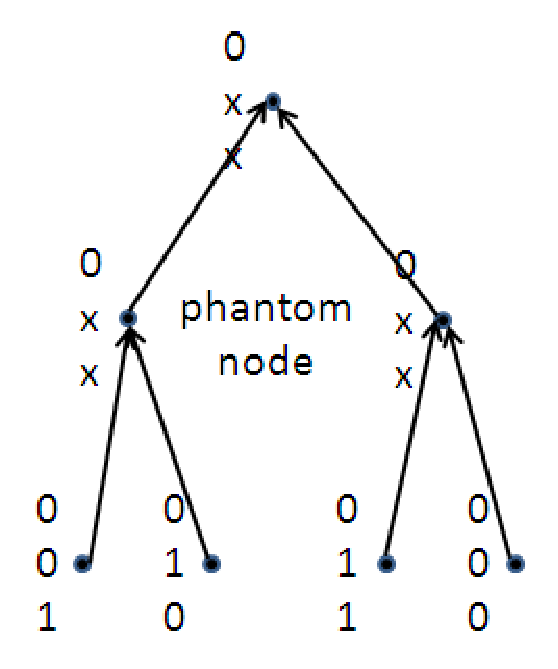
\includegraphics[scale=0.5]{figures/phantom_node.eps}
\caption{Phantom Nodes}
\label{fig:phantom-node}
\end{minipage}
\hspace{0.1cm}
\begin{minipage}[b]{0.3\linewidth}
\centering
\begin{tabular}{c|ccc}
$\otimes$ & 0 & 1 & x \\
\hline 
0 & 0 & x & x \\
1 & x & 1 & x \\
x & x & x & x 
\end{tabular}
\caption{Truth table for $\otimes$ operation}
\label{fig:truth-table}
\end{minipage}
\hspace{0.1cm}
\begin{minipage}[b]{0.3\linewidth}
\centering
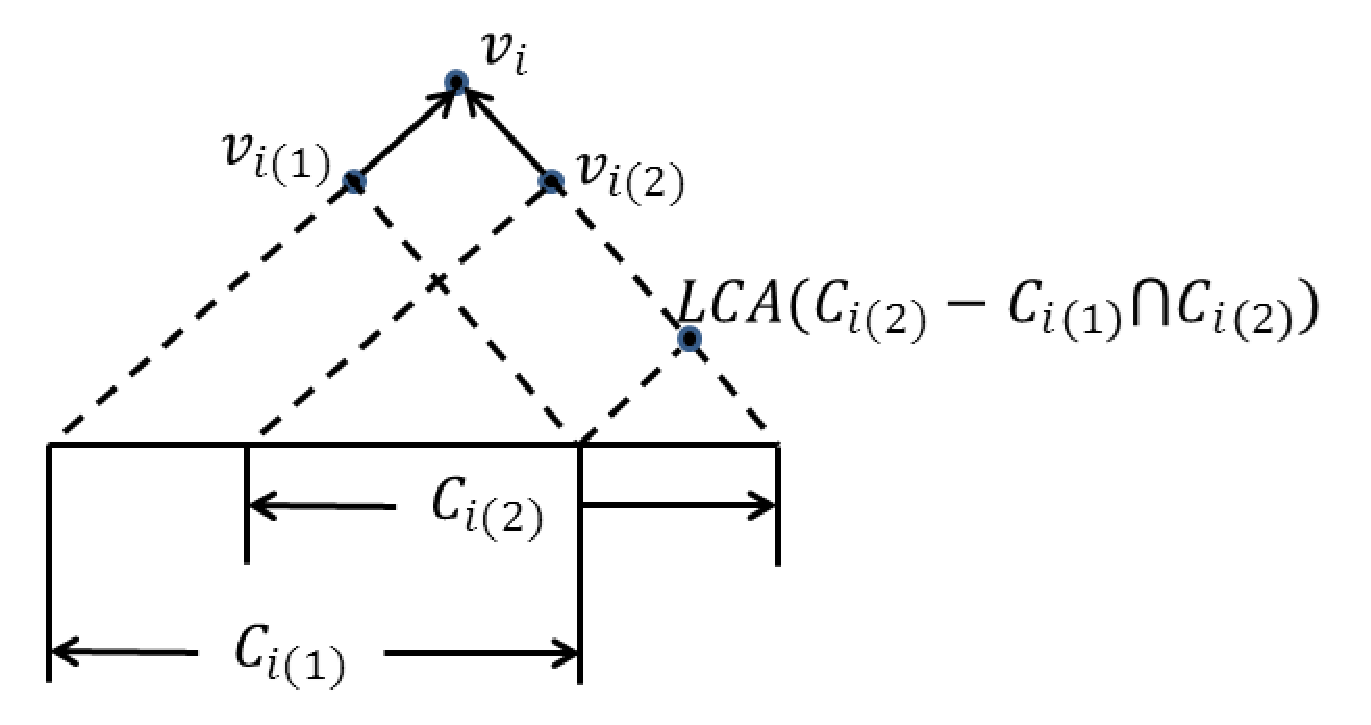
\includegraphics[scale=0.3]{figures/dag-overlap.eps}
\caption{Illustration of how to handle overlap}
\label{fig:dag-overlap}
\end{minipage}
\end{figure}

%This new algorithm adopts Charles' mechanism of FIFO to generate all
%unified columns
\begin{itemize}
    \item Prepare $g+1$ bins, i.e. $\{0, 1, \ldots, g\}$. Each bin $i$
    ($i \in [0, g]$) will correspondingly contains all columns that
    derived from original $m$ input columns and have $i$ ``x''s.

    \item Prepare a {FIFO} queue and put all initial $m$ input columns 
    into the {FIFO} queue. 

    \item Each time, remove a head element (column) from the {FIFO}
    queue, apply it with $\otimes$ operation to the rest of elements
    (columns) in the {FIFO} and insert resulting unified elements (columns)
    into the {FIFO} queue. After applying the head element to all
    the rest elements in {FIFO}, insert the head element into bin $i$
    according to how many ``x'' it has in it form.

\end{itemize}

\begin{theorem}
If assuming the number of initial input columns is $m$, the number of
total resulting unified (by $\otimes$ operation) but different columns
is $M$, then the total number of $\otimes$ operation is at most $O(M^2)$.
\label{thm:totalNodes}
\end{theorem}

\begin{IEEEproof}
Since the total number of elements (columns) in the {FIFO} queue is at
most $M$ at any moment, and each element will $\otimes$ with the rest
of elements in {FIFO} queue, so it's at most $O(M^2)$ times.
\end{IEEEproof}

\punt{%
    %for this old version, the conjecture that we only need to merge
    %columns in the same bin to produce all possible combinations of
    %medians (unified columns) is NOT true
\begin{itemize}

    \item Prepare $g+1$ bins, i.e. $\{0, 1, \ldots, g\}$. Each bin $i$
    ($i \in [0, g]$) will correspondingly contains all columns that
    derived from original $m$ input columns and have $i$ ``x''s.

    \item Initially, assuming all columns contain no ``x''s so that
    we put all nodes into bin $0$.

    \item Merge all ${m \choose 2}$ possible pairs in bin $0$, spread
    resulting nodes into bins $1, 2, \ldots, g$, respectively, according
    to the number of ``x''s appeared in merged nodes. E.g. if we merge
    column $(0, 1, 0)^T$ and column $(0, 1, 1)^T$, we get a new node
    $(0, 1, x)^T$ and it will go into bin $1$. If we merge node $(0,
    1, 0)^T$ and node $(0, 0, 1)^T$, we get a new node $(0, x, x)^T$
    and it should go to bin $2$, and so on.  In addition, for each node
    $v_i$, we associate it with a tuple $(\mathcal{C}_i, h_i)$, where
    $\mathcal{C}_i$ is the set of original input nodes that are leaves of
    the sub-tree rooted at node $v_i$, $h_i$ is the height of node $v_i$
    and equals to the number of ``x''s appeared in the new node.

    \item Since every non-leaf node is merged from two nodes in the lower
    level bins, if more than $1$ pair of nodes merged into the same node,
    we make a phantom node (see~\figref{phantom-node}), which has the same
    node signature, so as to make each node in the hierarchical {DAG}
    has two and only two children. It's easy to prove that if the old {DAG} 
    has $M$ nodes in total, after augmenting with phantom nodes, the new 
    {DAG} will have $\leq 2M$ nodes. Basically, the idea is to transform
    a non-binary tree to a binary tree by augmenting with phantom nodes.

    \item For bin $i$, we merge all ${bin(i) \choose 2}$ node
    combinations , spread the resulting nodes to bin $i+1, i+2, \ldots,
    g$, respectively, depending on the number of ``x''s appeared
    in merged nodes. Any collision of new nodes in any bins will be
    discarded due to redundancy.  We have the observation
    that for the ``merge'' operation, properties of idempotence, 
    associativity, and commutativity hold,
    i.e., for any node in bin $i$ that merged from input columns $\id{c_0},
    \id{c_1}, \ldots, \id{c_i}$, can be generated from two nodes
    in bin $i-1$ that merged from input columns $\id{c_0}, \id{c_1},
    \ldots, \id{c_{i-1}}$, and input columns $\id{c_1}, \id{c_2},
    \ldots, \id{c_{i}}$, respectively.

    \item Repeat above procedure at most $g$ iterations or until no
    bins have any increments of new nodes. 

\end{itemize}
} %end punt

\subsecput{stage2}{Compute the $k$-medians out of the hierarchical {DAG}}
In stage $2$, we need to compute a $k$-medians on $T$.

\begin{itemize}

    \item Naively, ${bin(0) + bin(1) + \ldots + bin(g) \choose k}$
    will be our global optimum. But this method will yield complexity
    bound ${M \choose k} = O(M^k)$.

    \item Another way to compute the $k$-medians out of the hierarchical
    {DAG} is via dynamic programming. Following algorithm to compute
    $k$-medians on the hierarchical {DAG} is largely adapted from the
    algorithm in \cite{Tamir96}. The algorithm in \cite{Tamir96} computes
    $k$-medians on a tree with $n$ nodes in time $O(kn^2)$.  For trees,
    any two sub-trees don't overlap with each other, but for {DAG}s, any
    two sub-trees can overlap. So the innovation of following algorithm
    lies in mostly how to handle overlaps.

        \begin{itemize}
        
            \item Define $d(\mathcal{V}_j) = d(\mathcal{C}_j) =
            h_j \times \sum_{c_{j,i} \in \mathcal{C}_j} c_{j, i}$,
            where $h_j$ is the height / bin number of root node $v_j$,
            $\mathcal{C}_j$ is the set of all input columns that can
            be covered in tree $T_{v_j}$, and $c_{j, i}$ are elements
            of set $\mathcal{C}_j$.  Note that $\mathcal{C}_j$ is also
            the set of leaves of tree $T_{v_j}$

            \item Define $d(\mathcal{V}_i) \oplus d(\mathcal{V}_j) = d(\mathcal{C}_i) \oplus d(\mathcal{C}_j) = 
            h_i \times \sum_{c_{i, l_i} \in \mathcal{C}_i 
                      \wedge c_{i, l_i} \notin \mathcal{C}_j} c_{i, l_i} + 
     \min \{h_i, h_j\} \times \sum_{c_{l_o} \in \mathcal{C}_i \cap \mathcal{C}_j} c_{l_o} +
            h_j \times \sum_{c_{j, l_j} \in \mathcal{C}_j 
                      \wedge c_{j, l_j} \notin \mathcal{C}_i}$.

            \item Define $\otimes$ to be a bit-wise operation depending
            on truth table of~\figref{truth-table}. So, $\mbox{LCA}(v_i,
            v_j) = v_i \otimes v_j$.

            \item For each node $v_i$, an integer $q = 1, \ldots, k$,
            define $G(v_i, q)$ be the optimal value of the subproblem
            defined on the sub-tree $T_{v_i}$, given that a total of at
            least $1$ and at most $q$ nodes (medians) are selected in
            $T_{v_j}$. Of course, the function $G(v_i, q)$ is computed
            only for $q \leq |\mathcal{V}_i|$, where $|\mathcal{V}_i|$
            is the number of total nodes (not just input columns)
            contained in sub-tree $T_{v_i}$.

            \item Define $d(G(v_i, q)) = d(\mathcal{C}_{m_0}) \oplus
            \ldots \oplus d(\mathcal{C}_{m_{q-1}})$, where $m_0,
            \ldots, m_{q-1}$ are the $q$ medians selected in sets
            $\mathcal{V}_j$

        \end{itemize}


    \item following procedure employs dynamic programming technique
    to compute the function $G(v_j, q)$ bottom up the hierarchial
    {DAG} $T$

    \begin{itemize}

        \item Apparently for every node $v_i$ in $T$, we define 
        $G(v_i, 0) = \infty$.

        \item If $v_i$ is a leaf of $T$, then $G(v_i, 1) = 0$. 
        $G(v_i, q) = 0$, for any $q \geq 1$.

        \item If $v_i$ is a non-leaf of $T$, since every non-leaf
        has two and only two children, we denote $v_{i(1)}$ to be the
        left child and $v_{i(2)}$ to be the right child of $v_i$ 
        respectively. We have recurrence (see \figref{dag-overlap}):
        \begin{align}
        \begin{split}
        G(v_i, q) = \min \{ 
            \min_{\substack{
                       q_1 + q_2 = q\\
                        q_1 \leq |\mathcal{C}_{i(1)} - \mathcal{C}_{i(1)} \cap \mathcal{C}_{i(2)}|\\
                        q_2 \leq |\mathcal{C}_{i(2)}| }}
                  \{ d(G(\mbox{LCA}(C_{i(1)} - C_{i(1)} \cap C_{i(2)}), q_1)) \oplus 
                     d(G(v_{i(2)}, q_2))
                  \}\\
                      , \\
            \min_{\substack{
                       q_1 + q_2 = q\\
                        q_1 \leq |\mathcal{C}_{i(1)}|\\
                        q_2 \leq |\mathcal{C}_{i(2)} - \mathcal{C}_{i(1)} \cap \mathcal{C}_{i(2)}| }}
                  \{ d(G(v_{i(1)}, q_1))) \oplus 
                     d(G(\mbox{LCA}(C_{i(2)} - C_{i(1)} \cap C_{i(2)}, q_2))
                  \}\\
                      , \\
            d(\mathcal{V}_i) \oplus
            \min_{\substack{
                       q_1 + q_2 = q-1\\
                        q_1 \leq |\mathcal{C}_{i(1)} - \mathcal{C}_{i(1)} \cap \mathcal{C}_{i(2)}|\\
                        q_2 \leq |\mathcal{C}_{i(2)}| }}
                  \{ d(G(\mbox{LCA}(C_{i(1)} - C_{i(1)} \cap C_{i(2)}), q_1)) \oplus
                     d(G(v_{i(2)}, q_2))
                  \}\\
                      , \\
            d(\mathcal{V}_i) \oplus
            \min_{\substack{
                       q_1 + q_2 = q-1\\
                        q_1 \leq |\mathcal{C}_{i(1)}|\\
                        q_2 \leq |\mathcal{C}_{i(2)} - \mathcal{C}_{i(1)} \cap \mathcal{C}_{i(2)}|}}
                  \{ d(G(v_{i(1)}, q_1)) \oplus
                     d(G(\mbox{LCA}(C_{i(2)} - C_{i(1)} \cap C_{i(2)}), q_2))
                  \}\\
        \}
        \end{split}
        \label{eq:recG}
        \end{align}

        In recurrence \ref{eq:recG}, terms ``$ \min_{\substack{
                       q_1 + q_2 = q\\
                        q_1 \leq |\mathcal{C}_{i(1)} - \mathcal{C}_{i(1)} \cap \mathcal{C}_{i(2)}|\\
                        q_2 \leq |\mathcal{C}_{i(2)}| }}
                  \{ d(G(\mbox{LCA}(C_{i(1)} - C_{i(1)} \cap C_{i(2)}), q_1)) \oplus 
                     d(G(v_{i(2)}, q_2))
                  \}$''
                  and 
                  ``$ \min_{\substack{
                       q_1 + q_2 = q\\
                        q_1 \leq |\mathcal{C}_{i(1)}|\\
                        q_2 \leq |\mathcal{C}_{i(2)} - \mathcal{C}_{i(1)} \cap \mathcal{C}_{i(2)}| }}
                  \{ d(G(v_{i(1)}, q_1))) \oplus 
                     d(G(\mbox{LCA}(C_{i(2)} - C_{i(1)} \cap C_{i(2)}, q_2))
                  \}$''
        represent the case that all $q$ medians are selected in two sub-trees
        of the tree $T_i$. 

        Terms ``$d(\mathcal{V}_i) \oplus
            \min_{\substack{
                       q_1 + q_2 = q-1\\
                        q_1 \leq |\mathcal{C}_{i(1)} - \mathcal{C}_{i(1)} \cap \mathcal{C}_{i(2)}|\\
                        q_2 \leq |\mathcal{C}_{i(2)}| }}
                  \{ d(G(\mbox{LCA}(C_{i(1)} - C_{i(1)} \cap C_{i(2)}), q_1)) \oplus
                     d(G(v_{i(2)}, q_2))
                  \}$''
                  and 
            ``$d(\mathcal{V}_i) \oplus
            \min_{\substack{
                       q_1 + q_2 = q-1\\
                        q_1 \leq |\mathcal{C}_{i(1)}|\\
                        q_2 \leq |\mathcal{C}_{i(2)} - \mathcal{C}_{i(1)} \cap \mathcal{C}_{i(2)}|}}
                  \{ d(G(v_{i(1)}, q_1)) \oplus
                     d(G(\mbox{LCA}(C_{i(2)} - C_{i(1)} \cap C_{i(2)}), q_2))
                  \} $''
        represent the case that we select node $v_i$ as one of the 
        medians, and select the rest $q-1$ medians from two sub-trees.

    \end{itemize}
\end{itemize}

\subsecput{opt}{Proof of Global Optimality}
In this section, we are trying to prove that the $k$-medians got from
above algorithm are the global optimum.

\begin{theorem}
Let's denote $v_0$ to be the root of the {DAG} $T$, global $k$-median
optimum $G(v_0, k)$ can be given by any two non-overlapping sub-trees
which covers the entire set of $\mathcal{C}_0$ by recurrence
\ref{eq:recG}. That is, if $T_i$ and $T_j$ are two sub-trees of $T$,
$(\mathcal{C}_i \cup \mathcal{C}_j = \mathcal{C}_0) \wedge (\mathcal{C}_i \cap \mathcal{C}_j = \emptyset)$, then 
        $G(v_0, k) = 
            \min \{ \min_{\substack{
                       k_1 + k_2 = k\\
                        k_1 \leq |\mathcal{V}_i|\\
                        k_2 \leq |\mathcal{V}_j| }}
                  \{ d(G(v_i, k_1)) \oplus d(G(v_j, k_2)) \}
                      , 
            d(\mathcal{V}_0) \oplus
            \min_{\substack{
                       k_1 + k_2 = k-1\\
                        k_1 \leq |\mathcal{V}_i|\\
                        k_2 \leq |\mathcal{V}_j| }}
                  \{ d(G(v_i, k_1)) \oplus d(G(v_j, k_2)) \}
        \}$. In short, let's denote $G(v_0, k) = \min_{k_1 + k_2 = k}\{ \mathcal{C}_i \odot \mathcal{C}_j \}$
\end{theorem}

\begin{IEEEproof}
Let's prove the theorem by induction on the height $h$ of the {DAG}:

\begin{itemize}
\item When height of {DAG} equals $0$, i.e. $v_0$ is a leaf node, apparently
$G(v_0, q)$, where $q \in [0, k]$ gives the global optimum.

\item When height of {DAG} equals $1$, which means, for non-leaf node $v_0$,
its only two sub-trees are leaves. Since it's binary tree and both its
sub-trees are leaves and non-overlapping, $G(v_0, q)$,
where $q \in [0, 3]$ gives the global optimum.

\item Assuming that for any {DAG} of height $h$, the conclusion holds.

\item For {DAG} $T_0$ of height $h+1$. If we divide $\mathcal{C}_0$ into
two disjoint sub-sets $\mathcal{C}_i$ and $\mathcal{C}_j$, apparently,
the corresponding $G(v_i, k_1)$, where $k_1 \leq |\mathcal{V}_i|$, 
and $G(v_j, k_2)$, where $k_2 \leq |\mathcal{V}_j|$ gives corresponding 
global optimum of two sub-trees $T_i$ and $T_j$. Now, we are going to 
prove that $G(v_0, k) = \min_{k_1 + k_2 = k}\{ \mathcal{C}_i \odot \mathcal{C}_j \}$ gives the global optimum of tree $T_0$. 

        Suppose it's not, which means that at least there is one median
        $m_k$ not in sub-trees $T_i$ or $T_j$. Since $\mathcal{C}_i \cup \mathcal{C}_j = \mathcal{C}_0$, so we can divide the input column set $\mathcal{C}_{m_k}$ of $T_{m_k}$ into two disjoint sets $\mathcal{C}_{m_k, i}$ and $\mathcal{C}_{m_k, j}$,
        such that $(\mathcal{C}_{m_k, i} \cup \mathcal{C}_{m_k, j} = \mathcal{C}_{m_k}) \wedge (\mathcal{C}_{m_k, i} \subseteq \mathcal{C}_i) \wedge (\mathcal{C}_{m_k, j} \subseteq \mathcal{C}_j)$. So, we can further divide $\mathcal{C}_i$
        into two sub-sets $\mathcal{C}_{m_k, i} \cup (\mathcal{C}_i - \mathcal{C}_{m_k, i})$, and divide $\mathcal{C}_j$ into two sub-sets $\mathcal{C}_{m_k, j} \cup (\mathcal{C}_j - \mathcal{C}_{m_k, j})$, respectively.

        According to the inductive hypothesis, $G(v_{m_k}, k) = \min_{k_1 + k_2 = k} \{ \mathcal{C}_{m_k, i} \odot \mathcal{C}_{m_k, j}\}$, 
        $G(v_i, k) = \min_{k_1 + k_2 = k}\{\mathcal{C}_{m_k, i} \odot (\mathcal{C}_{i} - \mathcal{C}_{m_k, i})\}$,
        $G(v_j, k) = \min_{k_1 + k_2 = k}\{\mathcal{C}_{m_k, j} \odot (\mathcal{C}_{j} - \mathcal{C}_{m_k, j})\}$.
        So, any benefits can be got from median $m_k$ must be already
        covered by two non-overlapping sub-trees $T_i$ and $T_j$.
\end{itemize}
\end{IEEEproof}

\secput{example}{Example}

Assuming we have input bit-matrix as follows ($3$ rows, $5$ columns):

\[ 
\begin{pmatrix} 
0 & 0 & 0 & 1 & 1 \\
0 & 0 & 1 & 0 & 1 \\
0 & 1 & 0 & 0 & 1 \\
\end{pmatrix}
\]

So it has $5$ input columns, $g = 3$.

After stage $1$, it has following bins:

\begin{figure}[!h]
\begin{minipage}[b]{0.5\linewidth}
\centering
\begin{tabular}{|c|ccccc|}
\hline
bin 1 & column 0 & column 1 & column 2 & column 3 & column 4 \\
\hline
00x & 1 & 1 & $\infty$ & $\infty$ & $\infty$ \\
0x0 & 1 & $\infty$ & 1 & $\infty$ & $\infty$ \\
x00 & 1 & $\infty$ & $\infty$ & 1 & $\infty$ \\
\hline
bin 2 & column 0 & column 1 & column 2 & column 3 & column 4 \\
\hline
0xx & 2 & 2 & 2 & $\infty$ & $\infty$ \\
x0x & 2 & 2 & $\infty$ & 2 & $\infty$ \\
xx0 & 2 & $\infty$ & 2 & 2 & $\infty$ \\
xx1 & $\infty$ & 2 & $\infty$ & $\infty$ & 2 \\
x1x & $\infty$ & $\infty$ & 2 & $\infty$ & 2 \\
1xx & $\infty$ & $\infty$ & $\infty$ & 2 & 2 \\
\hline
bin 3 & column 0 & column 1 & column 2 & column 3 & column 4 \\
\hline
xxx & 3 & 3 & 3 & 3 & 3 \\
\hline
\end{tabular}
\caption{Generated data structure in bins}
\label{fig:bin}
\end{minipage}
\hspace{0.2cm}
\begin{minipage}[b]{0.5\linewidth}
\centering
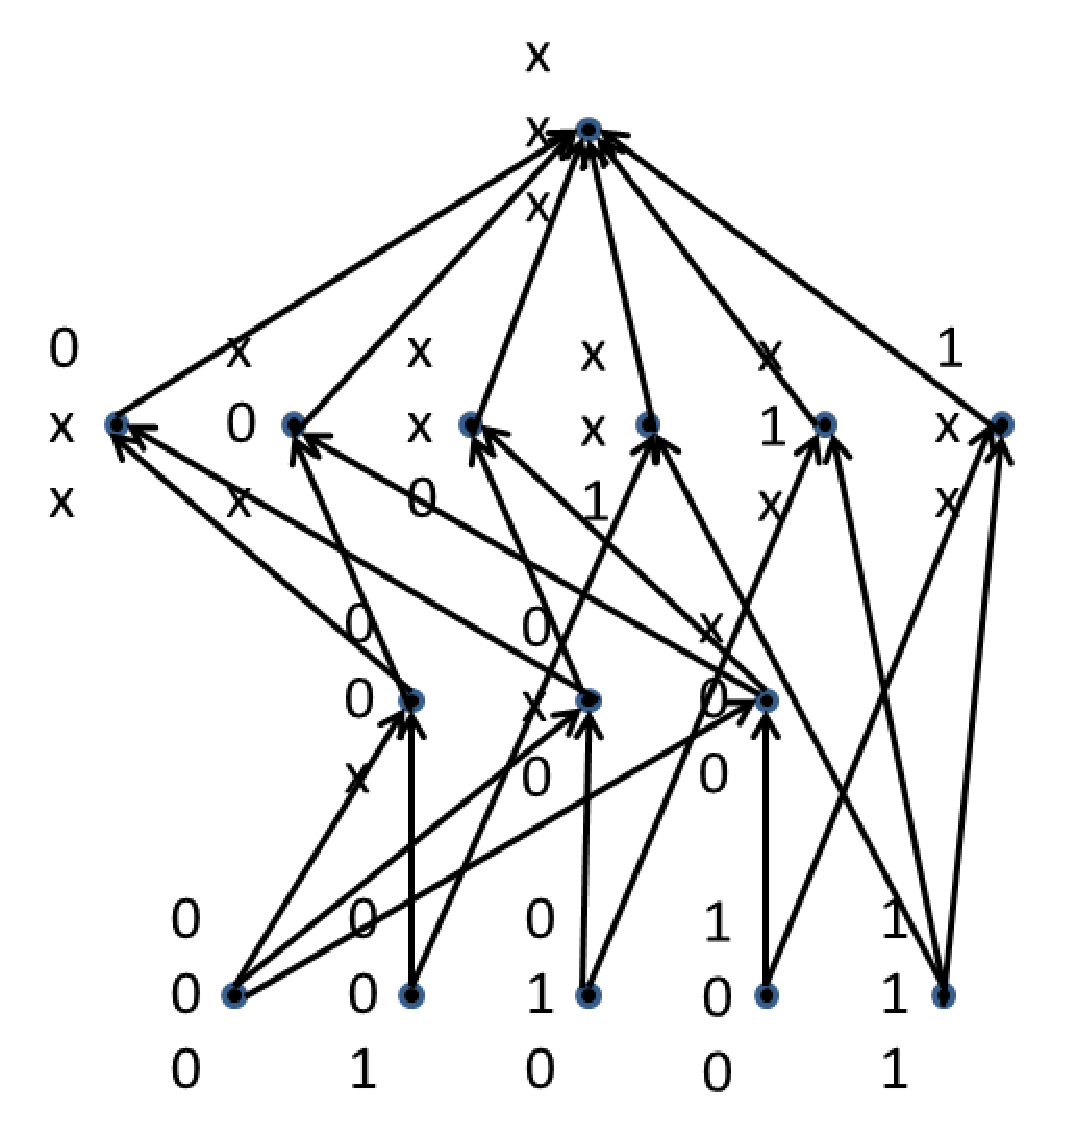
\includegraphics[scale=0.5]{figures/dag.eps}
\caption{Generated {DAG} data structure}
\label{fig:dag}
\end{minipage}
\end{figure}

From ~\figref{bin}, we can see that from $5$ input columns, the algorithm will
generate $10$ new nodes spreaded in $3$ different bins.  If including
the input $5$ columns, the {DAG} has $15$ total nodes as illustrated
in \figref{dag}.

\secput{analysis}{The Analysis of Complexity Bound}

\subsecput{stage1Analysis}{The complexity bound of stage $1$}
From \thmref{totalNodes} we can see that if we assume the {DAG} has $M$
nodes, the algorithm to construct the {DAG} is no more than $M^2$. In
this section, we are going to clarify the relation of $M$ and the number
of input columns $m$.

Intuitively, $m \in [2, 2^g]$, when $m = 2$, $M = 3 \in O(m^2)$, when 
$m = 2^g$, $M = 3^g = O(m^2)$, also, if $M = f(m)$, this $f$ seems an 
monotonically increasing function. However, it turns out that in the 
worst case, $M$ can be an exponential of $m$. Following theorem tries to 
prove it by induction.

\begin{theorem}
If there are $m$ input columns, each of which is of $g$ bit wide. If we
assume the output {DAG} has $M = f(m)$ nodes in total (including the
input $m$ columns), then in the worst case $M = f(m) = O(2^g)$.
\label{thm:worstCaseM}
\end{theorem}

\begin{IEEEproof}
Actually, the worst case comes when the input bit matrix is diagonal 
as follows: 

\[
\begin{pmatrix}
1 & 0 & \cdots & 0 \\
0 & 1 & \cdots & 0 \\
\vdots & \vdots & \ddots & \vdots \\
0 & 0 & \cdots & 1
\end{pmatrix}
\]

If we induct on the number of input columns, we have:

First, for $m = 2$, $M = 3$. 

Second, if assuming that we already constructed a {DAG} from $m$
input columns, $c_0, c_1, \ldots, c_{m-1}$, and bin $0$ has $b_0 = m$
nodes, bin $1$ has $b_1$ nodes, $\ldots$, bin $i$ has $b_i$ nodes. When we
add in one more node $c_m$, let's count how many nodes will be increased
in each bin, and total.

\begin{itemize}

\item for bin $0$, apparently, $b_0' = b_0 + 1$. 

\item for bin $1$, $b_1' = b_1 + b_0$. The new nodes in bin $1$ are of
the form $c_i c_m$, with $c_i \in$ bin $0$. Because it's diagonal matrix,
so the newly add-in node $c_m$ has a $1$ set at different position from
any of existing old nodes, so there is no collision of newly merged nodes
with old nodes.

\item for bin $2$, $b_2' = b_2 + b_1$. Note that the new nodes in bin $2$ 
are of the form $c_i c_j c_m$, with $c_i, c_j \in b_1$.

\item for bin $i$, $b_i' = b_i + b_{i-1}$.

\item Overall, $\sum_i b_i' = 2 \sum_i b_i$, i.e. the summation of number
of nodes in all bins increases exponentially in this case. Because the
number of columns of diagonal matrix is at most $g$, so it has at most
$2^g$ nodes in all bins after the construction.

\end{itemize}
\end{IEEEproof}

\thmref{worstCaseM} is about the complexity of $M$ in the worst case,
following calculation yields the expected number of $M$.

\begin{eqnarray*}
E[bin(0)] & = & m \\
E[bin(1)] & = & {m \choose 2} \cdot \id{Pr}{\{I_{i, j}\}} \quad \mbox{where $I_{i, j} = 1$ if column $i$ and $j$ differs by only $1$ bit, $0$ otherwise} \\
       & = & {m \choose 2} \cdot \frac{{g \choose 1}}{2^g} \\
       & = & O(gm^2 / 2^g) \\
E[bin(2)] & = & {E[bin(1)] \choose 2} \cdot \id{Pr}{\{I_{i, j}\}} \quad \mbox{where $I_{i, j} = 1$ if column $i$ and $j$ differs by only $1$ non-``x'' position, $0$ otherwise } \\
       & = & (\frac{gm^2}{2^g})^2 \cdot \frac{g-1}{2^{g-1}} \\
       & = & O(\frac{g^3 m^4}{2^{3g}}) \\
\ldots & = & \ldots \\
E[bin(i)] & = & {E[bin(i-1)] \choose 2} \cdot \id{Pr}{\{I_{i, j}\}} \quad \mbox{where $I_{i, j} = 1$ if column $i$ and $j$ differs by only $1$ non-``x'' position, $0$ otherwise } \\
       & = & O(\frac{g^{2i-1} \cdot m^{2^i}}{2^{(2i-1)g}})
\end{eqnarray*}

By non-``x'' position, we distinguish two cases: 

\begin{itemize}

    \item columns $(0, 1, 0)^T$ and $(0, 1, x)^T$ differ by a ``x'' position.

    \item columns $(0, 0, 0)^T$ and $(0, 1, x)^T$ differ by a non-``x'' position.
\end{itemize}

So, $E[\sum_{i=0}^{g} |bin(i)|] = O(\frac{g^{2g} \cdot m^{2^g}}{2^{2g^2}})$

\subsecput{stage2Analysis}{The complexity bound of stage $2$}
Apparently, in recurrence~\ref{eq:recG}, operation ``$\mbox{LCA}$'' has
complexity $O(m)$, set operation ``$-$'' and ``$\cap$'' has complexity
$O(m)$, ``$\oplus$'' has complexity $O(m)$. The recurrence~\ref{eq:recG}
takes a minimum of four terms, each of which has complexity $O(qm)$. If
we assume there are total $M$ nodes in {DAG} $T$, in total, the complexity
is $O(M \sum_{q = 1}^{k} qm) = O(k^2 M m)$.

\punt{%
\subsecput{totalComplexity}{Overall complexity of the algorithm}
From stage $1$, we have $M = O(m^2)$. From stage $2$, we have complexity
$O(k^2 M m)$. So combine these two, we have overall complexity $O(k^2 m^3)$
for the algorithm.
} % end punt

\secput{ext}{Extension the code-clone selection puzzle from point to region}

The extension of code-clone selection puzzle from point to region is 
straightforward. The differences are

\begin{itemize}
\item The entry in bit-matrix can be 'x'. $\{0, 1, x\}$

\item The 'x' in bit-matrix comes from contraction of a whole region to 
one bit-vector via bit-wise operation $\otimes$

\item After this contraction, each bit-vector will be associated with
a weight $w_i$ to denote the number of points it represents.

\item In computing the $k$-medians out of the {DAG}, we also need to 
take the weights of each node into account. 
\end{itemize}

But the basic algorithm and complexity bound shouldn't change.

% introduce the concept of meta-algortihm and how to perform orthogonal
% query for d-dimensional grid, including parallelization as a sub-section
% introduce how to perform irregular range query by meta-algorithm
% % -*- Mode: LaTeX -*-
\secput{future}{Future Work}

Some possible future work may be:

\begin{itemize}
    \item How to relax the current constraints on polygonal range queries
    in $2$-D grids, such as arbitrary triangular queries.
    \item How to extend the polygonal range query in $2$-D to polytopal 
    range query in $3$-D grids.
\end{itemize}

\punt{In this paper, we developed a data reduction method, developed a
meta-algorithm $M$ for the partial sum query problem over $d$-dimensional
array ($d \geq 1$) of size $N$. Provided the partial sum operation is
valid over a semi-group and is associative and commutative, by taking
a user's input preprocessing algorithm $P$ of complexity $\Theta(N
\log^p N)$ in both space and time, where $0 \leq p \leq d$, and query
algorithm $Q$ of complexity $q(N, d)$, the meta-algorithm will output
a preprocessing algortihm $M(P)$ of complexity $\Theta(N \log^{p-1}
N)$,  a query algorithm $M(Q)$ with complexity $\Theta(2^{2d \cdot
\log^{*} N} \cdot q(N, d))$. Moreover, since the meta-algorithm treats
the input algorithm as a black box, if we view the meta-algorithm as a
higher-order function, by applying $M$ to $P$ at most $p$ times, i.e.
$\underbrace{M(M(\ldots M}_{p}(P)))$, we can reduce the preprocessing
complexity to optimal ($\Theta(N)$), with near-constant factor penalty on
query time (which can possibly be improved either by employing a similar
trick in \cite{AmirFiLe07} or by exploiting the internal structure of
the input query algorithm).  In addition, the result algorithm produces
good memory locality with an asymptotically smaller cache-oblivious
data structrure.}

 
% \section*{Acknowledgments}

TBD.


\bibliographystyle{IEEEtran}
\bibliography{allpapers}

% \appendix
% \secput{appendix}{Appendix}

\subsecput{apdx-meta-intro}{Meta-algorithm for $2$-D grids} 

From the results in \cite{Yao82, Yao85, Seidel06}, we can establish
following recurrence for space and time bound of $1$-D
preprocessing algorithm.

\begin{eqnarray}
\mathcal{S}_{1, 0} (n) & = & n \log n \hfil \mbox{// initial algo} \\
\mathcal{S}_{1, 1} (n) & = & \Theta(n) + \mathcal{S}_{1, 0}(n/\log n) + n/\log n \cdot \mathcal{S}_{1, 1}(\log n) \hfil \mbox{// use $\mathcal{S}_{1, 0}$ inter-block query}\\
\ldots & = & \ldots \\
\mathcal{S}_{1, k} (n) & = & \Theta(n) + \mathcal{S}_{1, k-1}(n / f(n)) + n/f(n) \cdot \mathcal{S}_{1, k}(f(n)) \hfil \mbox{// Suppose the complexity of $\mathcal{S}_{1, k-1}(n) = n f(n)$} \\ 
\mathcal{S}_{1, \alpha(n)} (n) & = & \Theta(n \alpha (n)) \\ 
\label{eq:meta-1D-S1}
\end{eqnarray}

For the notation $\mathcal{S}_{d, k}$, $\mathcal{S}$ stands for the
space and time bound, the first subscript stands for dimensionality,
the second is the recursion level. Similarly, we have a recurrence
for query overhead, where $\mathcal{Q}$ stands for the query overhead,
the semantics of subscript is the same as in $\mathcal{S}_{d, k}$:

\begin{eqnarray}
\mathcal{Q}_{1, 0} & = & 1 \hfil \mbox{// initial algo}\\
\mathcal{Q}_{1, 1} & = & 2 + \mathcal{Q}_{1, 0} \hfil \mbox{// any query can be decomposed into at most one inter-block query and one suffix/prefix} \\
\ldots & = & \ldots \\
\mathcal{Q}_{1, k} & = & 2 + \mathcal{Q}_{1, k-1} \\
\mathcal{Q}_{1, \alpha(n)} & = & \Theta(\alpha(n))
\label{eq:meta-1D-Q1}
\end{eqnarray}

To extend the same kind of recurrence to multi-dimensional grids,
we start from how to use meta-algorithm to process a $2$-D
grid and iteratively apply to itself to achieve alpha bound. 
First, we need an initial algorithm to kick
off. The initial algorithm doesn't need to be very smart, it just needs
to work. Our meta-algorithm will later transform it through a series
of recursion levels and improves the asymptotic bound to eventually hit
the alpha bound.

\subsubsecput{apdx-init-2D}{Initial algorithm for $2$D grids}

\begin{figure*}[!ht]
\centering
\subfigure[Initial algorithm for $2$D orthogonal range queries]{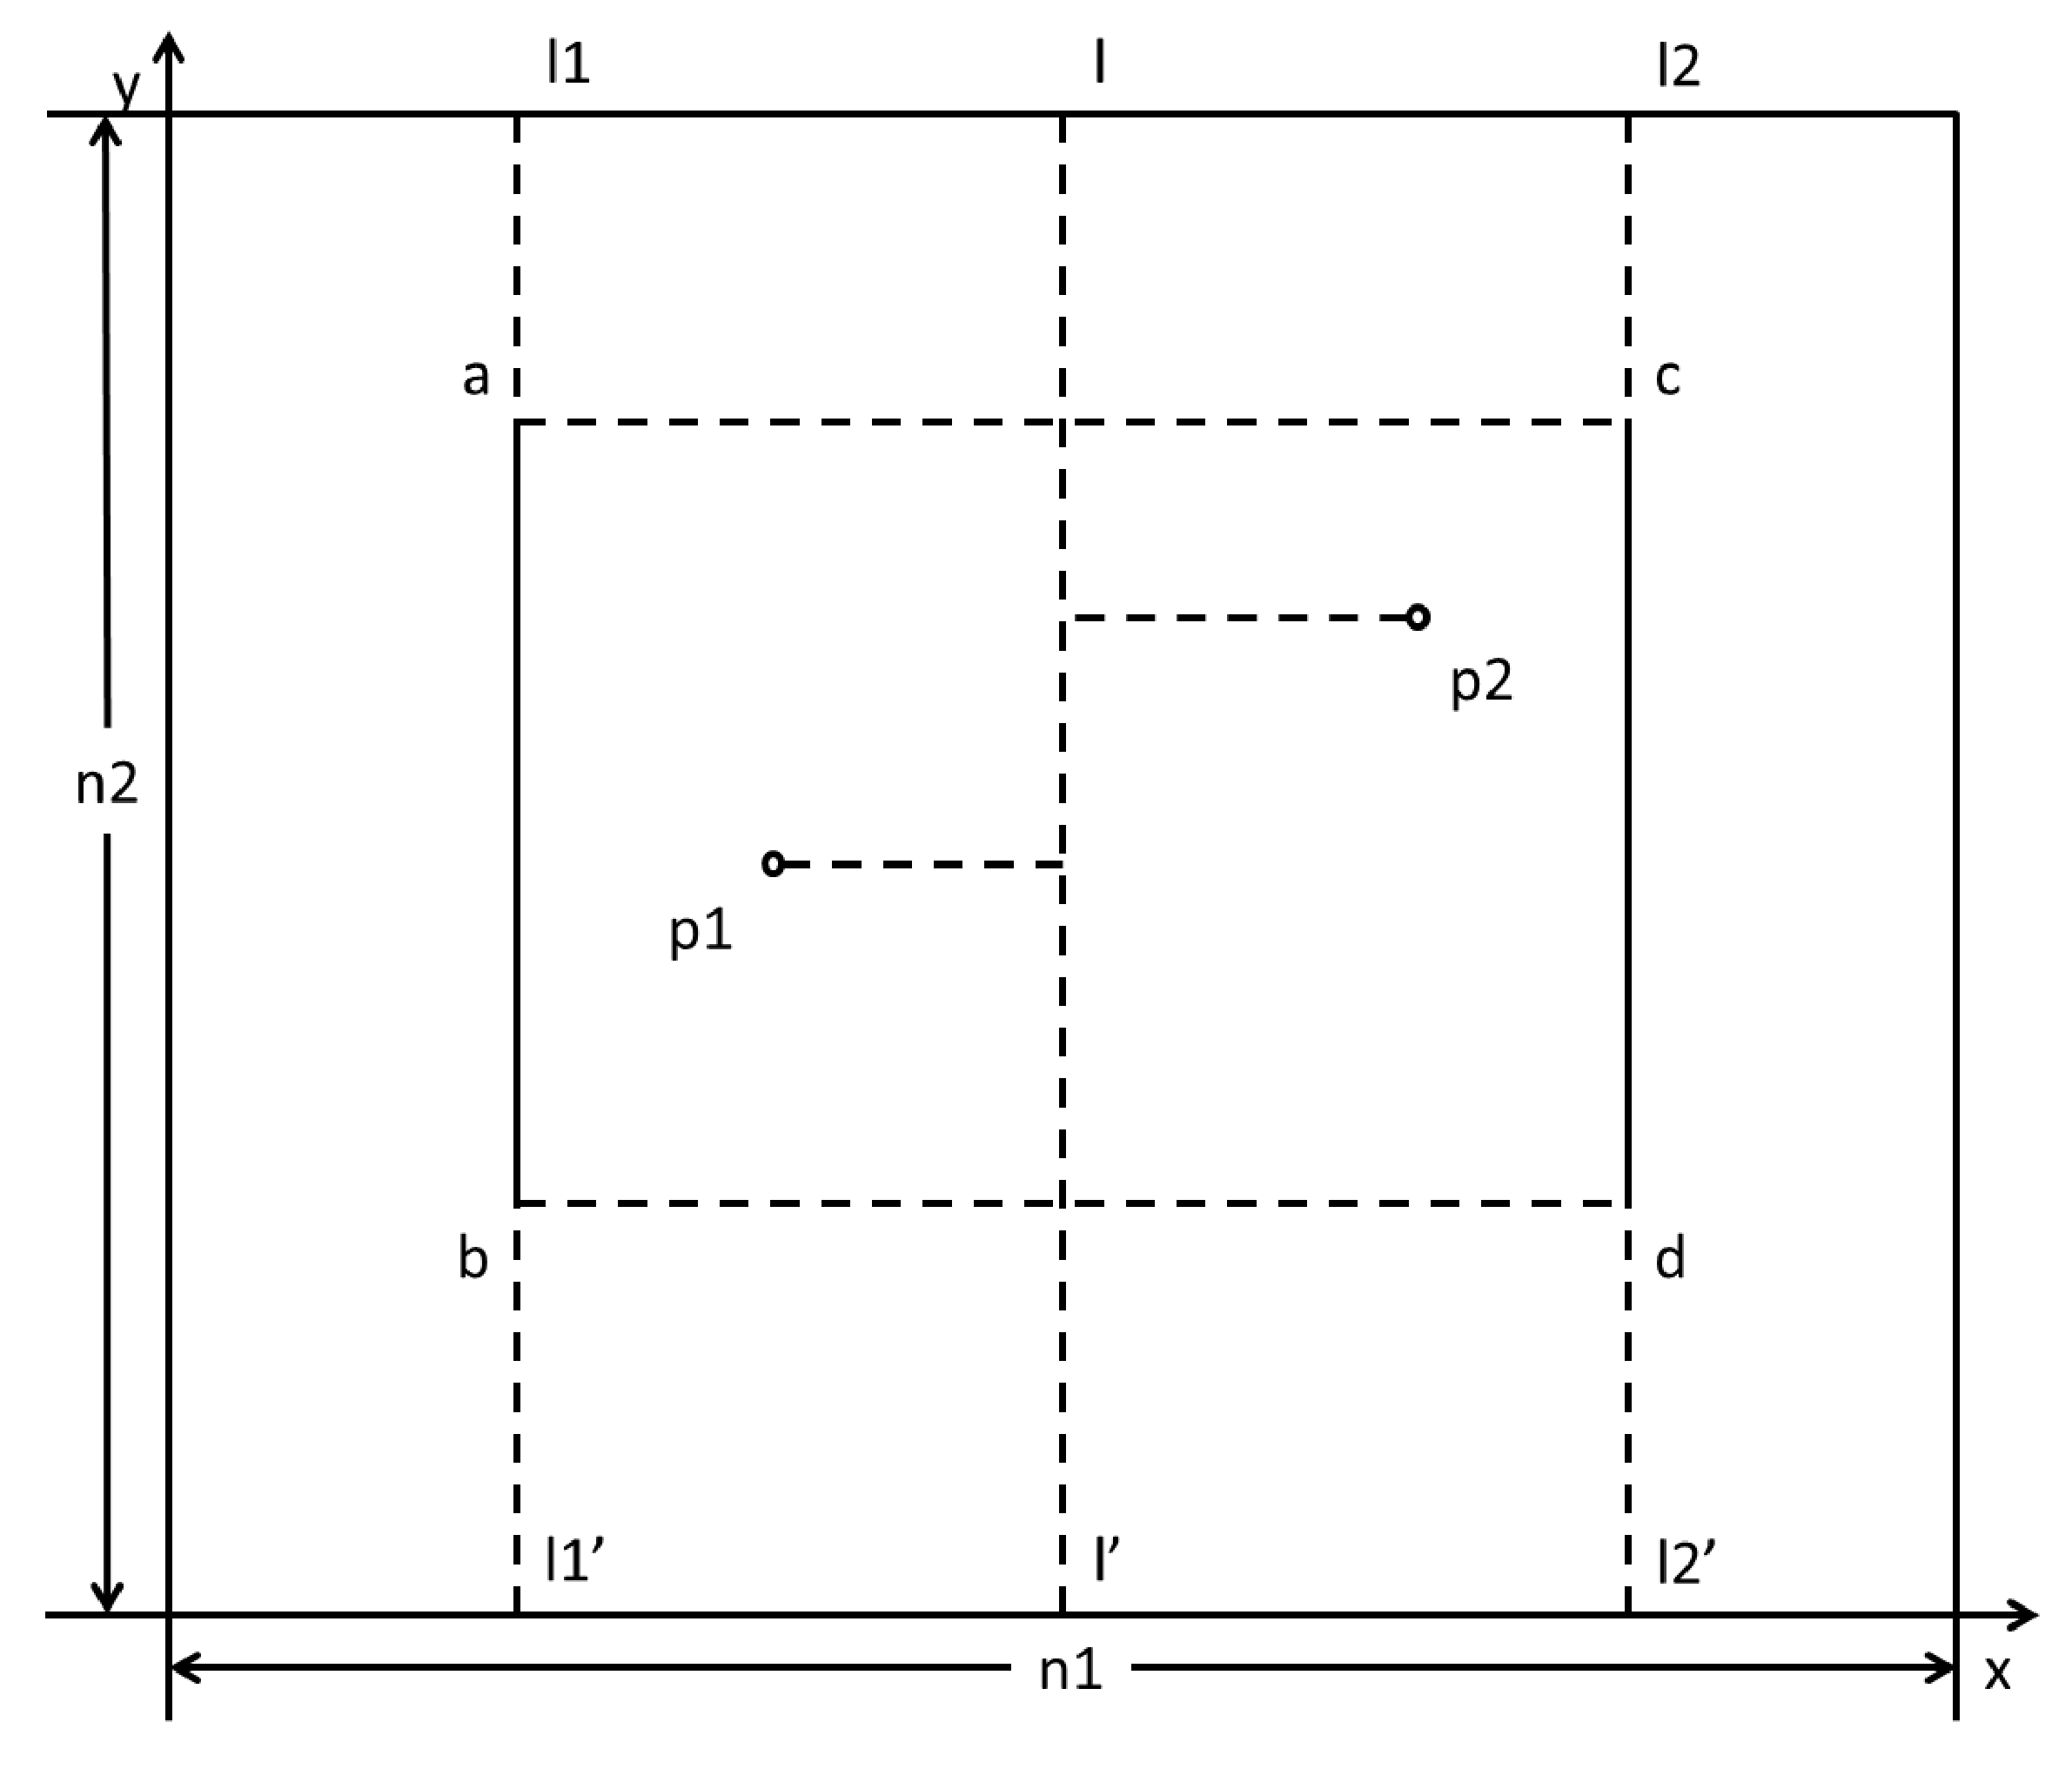
\includegraphics[clip,width=3in]{figures/init_2D.eps}
\label{fig:init-2D}}
\hfill
%\hspace{0.01cm}
\subfigure[Meta-algorithm for $2$D orthogonal range queries]{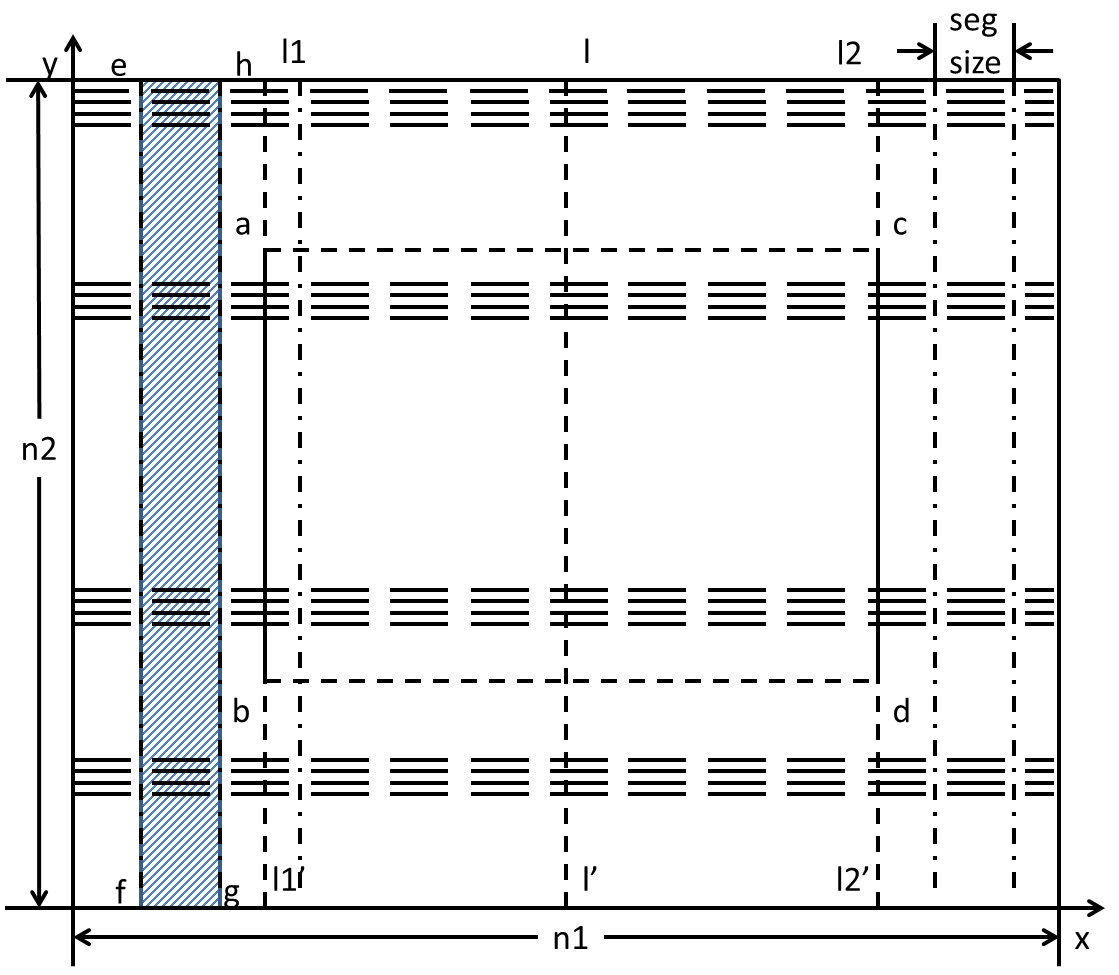
\includegraphics[clip,width=3in]{figures/meta_2D.eps}
\label{fig:meta-2D}
}
\caption{Initial and meta-algorithm for $2$-D orthogonal range queries}
\label{fig:twod}
\end{figure*}

As shown in \figref{init-2D}, the initial algorithm is a direct extension
of A. Yao's initial algorithm \cite{Yao82} to $2$-D grids. The algorithm
is diagrammed in \figref{init-2D}. The description is as follows and uses
the notation in \figref{init-2D}, the pseudo-code is in \figref{init-2D-algo}

\begin{enumerate}
\item Select a longer dimension, without loss of generality, let's
  suppose it's dimension $\id{x}$.
\item Partition dimension $\id{x}$ by a center line $\overline{\id{ll'}}$
  into evenly two parts. Then all points in the grid resides
  either on the left (e.g.  $\id{p_1}$) of the center line or right
  (e.g. $\id{p_2}$). For all the points, reducing (by applying the $\oplus$
  operator) the data from center line to itself by dynamic programming.
  We call the reduced data prefix or suffix value from the center line.
\item After data reduction on both prefix and suffix values, applying Yao's
  initial $1$-D preprocessing algorithm \cite{Yao82, ChazelleRo91},
  which has complexity $O(n \log (n))$ on all lines along vertical
  dimension $\id{y}$.
\item Now we have the observation that all $2$-D orthogonal range query
  that spans across the center line $\overline{\id{ll'}}$ can be
  answered by conducting two $1$-D queries on both left-hand side
  and right-hand side of the center line. E.g. To query the rectangle
  $\Box\id{abdc}$ in \figref{init-2D}, we perform one $1$-D query
  on line $\overline{\id{l_1l_1'}}$ and another $1$-D query on line
  $\overline{\id{l_2l_2'}}$. Combining these two results by $\oplus$
  operator, we get the final query result of the orthogonal range query.
\item Recursively applying the above procedure to the left and right
  sub-grids of line $\overline{\id{ll'}}$.
\end{enumerate}

\begin{theorem}
The preprocessing of Algoritm~\figref{init-2D} has complexity of
$\mathcal{S}_{2, 0}(n_1, n_2) = \Theta(n_1 \cdot n_2 \cdot \log (n_1)
\cdot \log(n_2))$ in both time and space.
\label{thm:init-2D-pp}
\end{theorem}

\begin{IEEEproof}
Apparently, at each level of recursion, it requires at least $n_1
n_2$ space and time to hold prefix and suffix grids.

For each vertical lines, such as $\overline{\id{l_1l_1'}}$ and
$\overline{\id{l_2l_2'}}$, we apply Yao's initial $1$-D algorithm on it, and
denote it as $\mathcal{S}_{1, 0}(n) = \Theta(n \log n)$. 

Since the partition occurs on dimension $\id{x}$, which will terminate
when the number of vertical lines in the grid less than or equal to $1$,
there are in total $\log n_1$ levels.

Combining all above calculations we have the recurrence:

\begin{eqnarray}
\mathcal{S}_{2, 0} (n_1, n_2) & = & n_1 n_2 + \log n_1 \{ n_1 \cdot \mathcal{S}_{1, 0}(n_2)\} \\
    & = & \Theta(\log n_1 n_1 n_2 \log n_2)
\label{eq:init-2D-S20}
\end{eqnarray}
\end{IEEEproof}

\begin{corollary}
The query overhead of Algorithm~\figref{init-2D} is 
$\mathcal{Q}_{2, 0} = 3-\oplus$
\label{cor:init-2D-query}
\end{corollary}

\begin{IEEEproof}
For the query, we first need to locate which recursion level the query
range resides, which is equivalent to finding the lowest common ancestor
of its range on dimension \id{x}, the overhead of which is not counted
in our simple arithmetic model.
\footnote{In RAM model, by using bit-tricks, finding lowest common
ancestor in a complete binary tree can be accomplished in $O(1)$ time} 

After locating the lowest common ancestor of the query range on dimension
\id{x}, performing two $1$-D queries on left and right-hand side of
the center line of the level, each of which requires 
$\mathcal{Q}_{1, 0} = 1-\oplus$
overhead. In the end, we need to combine both results from two $1$-D
queries into one, which requires another $1-\oplus$ operation. So in
total, we have $\mathcal{Q}_{2, 0} = 2 \mathcal{Q}_{1, 0} + 1 = 3$.
\end{IEEEproof}

\subsubsecput{apdx-meta-2D}{Meta-algorithm for $2$D grids}

The meta-algorithm takes an algorithm as input, such as the initial
algorithm described in ~\figref{init-2D} (\figref{init-2D-algo}),
compress the data alternatively on dimension $\id{x}$ or $\id{y}$ to
eventually hit the $\alpha$ bound. The description follows the notation
in \figref{meta-2D}, the pseudo-code is in \figref{meta-2D-algo}

\begin{enumerate}
\item We start data reduction on a longer dimension,
  without loss of generality, suppose it's dimension $\id{x}$. For
  each line of dimension $\id{y}$, partition it along dimension
  $\id{x}$ into segments of size $\log (\id{x_1} - \id{x_0})$, or
  $\log^* (\id{x_1} - \id{x_0})$, $\log^{**} (\id{x_1} - \id{x_0})$,
  $\ldots$ ($\id{seg\_size}$ in \figref{meta-2D-algo}). The length of
  $\id{seg\_size}$ depends on the complexity of $\id{input\_2D\_algo}$,
  which can be a user's input parameter.
\item For each segment, apply $\oplus$ operator over it and reduce
  all data within the segment into one single value. All such values
  construct a new grid --- $\id{promoted\_grid}$. Applying the
  $\id{input\_2D\_algo}$ to the $\id{promoted\_grid}$.
\item For each vertical line (along dimension $\id{y}$), reduce the
  the data relative to the left and right end of each segment (of
  size $\id{seg\_size}$ to construct the $\id{prefix\_grid}$ and
  $\id{suffix\_grid}$.
\item For each vertical line (e.g. line $\overline{l_1l_1'}$ and
  line $\overline{l_2l_2'}$ in \figref{meta-2D}) in $\id{prefix\_grid}$
  and $\id{suffix\_grid}$, apply the $\id{input\_1D\_algo}$ to it.
  If the $\id{input\_2D\_algo}$ has bound $\Theta(n_1 n_2 f_1(n_1)
  f_2(n_2))$, the corresponding $\id{input\_1D\_algo}$ should be of
  bound $\Theta(n f(n))$, where $f(n) \leq f_1(n)$ and $f(n) \leq f_2(n)$.
\item Recursively apply the meta-algorithm itself on segment blocks
  of size $\id{seg\_size} \times \id{n_2}$. E.g. on colored segment block
  $\Box \id{efgh}$ in \figref{meta-2D}
\item Repeat the above meta-algorithm alternatively on dimension
  $\id{y}$, $\id{x}$.
\end{enumerate}

\begin{theorem}
The preprocessing of Algoritm~\figref{meta-2D} has complexity of 
$\mathcal{S}_{2, \alpha(n_1) \alpha(n_2)} = \Theta(n_1
\cdot n_2 \cdot \alpha (n_1) \cdot \alpha(n_2))$ in both time and space.
\label{thm:meta-2D-pp}
\end{theorem}

\begin{IEEEproof}
\begin{enumerate}
\item In \thmref{init-2D-pp}, we proved that $\mathcal{S}_{2, 0} = 3$.
\item For recursion level $1$: we have $\mathcal{S}_{2, 0}$ as 
  $\id{input\_2D\_algo}$, and $\mathcal{S}_{1, 0}$ as $\id{input\_1D\_algo}$.
  We apply $\id{input\_2D\_algo}$ to $\id{promoted\_grid}$, which is
  of size $n_1/\log n_1 \times n_2$, and apply $\id{input\_1D\_algo}$
  to $\id{prefix\_grid}$ and $\id{suffix\_grid}$, each of which is of
  size $n_1 \times n_2$. So we have the recurrence:
    \begin{eqnarray}
      \mathcal{S}_{2, 1}(n_1, n_2) & = & \mathcal{S}_{2, 0} (n_1/\log n_1,
      n_2) + 2 \times n_1 \times \mathcal{S}_{1, 0} (n_2) 
      \frac{n_1}{\log n_1} \cdot \mathcal{S}_{2, 1}(\log n_1, n_2) \\
          & = & \Theta(n_1 n_2 \log n_2 \log^* n_1)
    \label{eq:meta-2D-S21} 
    \end{eqnarray} 
\item Solution in \eqref{meta-2D-S21} means we now have a $2$-D preprocessing
  algorithm of complexity $O(n_1 n_2 \log^* n_1 \log n_2)$ in both
  space and time. Repeat the same procedure on dimension $\id{y}$, we will 
  have the recurrence:
  \begin{eqnarray}
    \mathcal{S}_{2, 2}(n_1, n_2) & = & \mathcal{S}_{2, 1} (n_1, n_2/\log n_2) 
    + 2 \times n_2 \times \mathcal{S}_{1, 1} (n_1) 
    + \frac{n_2}{\log n_2} \cdot \mathcal{S}_{2, 2}(n_1, \log n_2) \\
        & = & \Theta(n_1 n_2 \log^* n_1 \log^* n_2) 
  \label{eq:meta-2D-S22}
  \end{eqnarray}
\item Repeat above two procedures, more generally, if we assume 
  $\id{input\_2D\_algo}$ has complexity $\Theta(n_1 n_2 f(n_1) f(n_2))$,
  where $f(n) \leq n-2$. We first segment the $2$-D grid along $\id{x}$
  dimension into size of $f(n_1)$ and supply a $1$-D algorithm of
  complexity $\Theta(n f(n))$, we will have the recurrence:
  \begin{eqnarray}
    \mathcal{S}_{2, k}(n_1, n_2) & = & \mathcal{S}_{2, k-1} (n_1/f(n_1), n_2)
    + 2 \times n_1 \times \mathcal{S}_{1, k-1} (n_2)
    + \frac{n_1}{f(n_1)} \cdot \mathcal{S}_{2, k}(f(n_1), n_2) \\
        & = & \Theta(n_1 n_2 f(n_2) f^*(n_1))
  \label{eq:meta-2D-S2k}
  \end{eqnarray}

  In a second step, we supply the $\mathcal{S}_{2, k}$ as 
  $\id{input\_2D\_algo}$ and a $1$-D algorithm of complexity 
  $\mathcal{S}_{1, k} = n f^*(n)$ as $\id{input\_1D\_algo}$.

  \begin{eqnarray}
    \mathcal{S}_{2, k+1}(n_1, n_2) & = & \mathcal{S}_{2, k} (n_1, n_2/f(n_2))
    + 2 \times n_2 \times \mathcal{S}_{1, k} (n_1) 
    + \frac{n_2}{f(n_2)} \cdot \mathcal{S}_{2, k+1}(n_1, f(n_2)) \\
        & = & \Theta(n_1 n_2 f^*(n_1) f^*(n_2))
  \label{eq:meta-2D-S2K1}
  \end{eqnarray}
\item We define the alpha function, i.e. the inverse Ackermann function to be:
  $\alpha(n) = min\{k \vert \log^{\overbrace{**\cdots*}^{k times}}(n) \leq 2\}$ 
  \cite{Seidel06}
\item Combining above steps completes the induction.
\end{enumerate}
\end{IEEEproof}

\begin{corollary}
Without loss of generality, if we assume $n_1 = n_2 = n = \sqrt(N)$, where
$N$ is the total number of points in entire grid.  The query overhead of
Algorithm~\figref{meta-2D} is $\mathcal{Q}_{2, k+1} = \Theta(\alpha^2(n))$
\label{cor:meta-2D-query}
\end{corollary}

\begin{IEEEproof}
For the query, we just need to locate which recursion level the query
range resides. At each level, the query will be decomposed into at most
three sub-queries, one $2$-D query on the $\id{promoted\_grid}$, two 
$1$-D queries on the $\id{prefix/suffix\_grid}$. If we assume that the
index calculation to locate the recursion level is free, we have following
recurrence for the query overhead:

\begin{eqnarray}
\mathcal{Q}_(2, 0) & = & 2 \times \mathcal{Q}_{1, 0} + 1 = 3 \hfil \mbox{//initial algorithm}  \\
\mathcal{Q}_(2, 1) & = & \mathcal{Q}_{2, 0} + 2 \times \mathcal{Q}_{1, 0} + 2 
    \hfil \mbox{//Decompose the query into one $2$-D query and two
    $1$-D queries} \\
\mathcal{Q}_{2, 2} & = & \mathcal{Q}_{2, 1} + 2 \times \mathcal{Q}_{1, 1} + 2 \\
\ldots & = & \ldots \\
\mathcal{Q}_{2, k}   & = & \mathcal{Q}_{2, k-1} + 2 * \mathcal{Q}_{1, k-1} + 2 \quad \mbox{//k is odd} \\
\mathcal{Q}_{2, k+1} & = & \mathcal{Q}_{2, k}   + 2 * \mathcal{Q}_{1, k} + 2 
\label{eq:meta-2D-query}
\end{eqnarray}
      
Solve the recurrence in \eqref{meta-2D-query}, we have $\mathcal{Q}_{2,
k+1} = 2 \Sigma_{i=0}^{k} \mathcal{Q}_{1, i} + 2 k$, where
$\mathcal{Q}_{1, k} = 2k + 1$ is the query overhead of $1$-D algorithm
\cite{Seidel06}.  So $\mathcal{Q}_{2, k+1} = 2 k (k+1) + 2k = \Theta(k^2)$
is the query overhead of the $2$-D meta-algorithm. Since the $1$-D
algorithm's query overhead is $\Theta(2 \alpha(n) + 1)$ \cite{Yao82,
Seidel06}, so the $2$-D meta-algorithm is $\Theta(\alpha^2(n))$
\end{IEEEproof}

\subsubsecput{apdx-init-3D}{Initial algorithm for $3$D grids}

\begin{figure}[!ht]
\centering
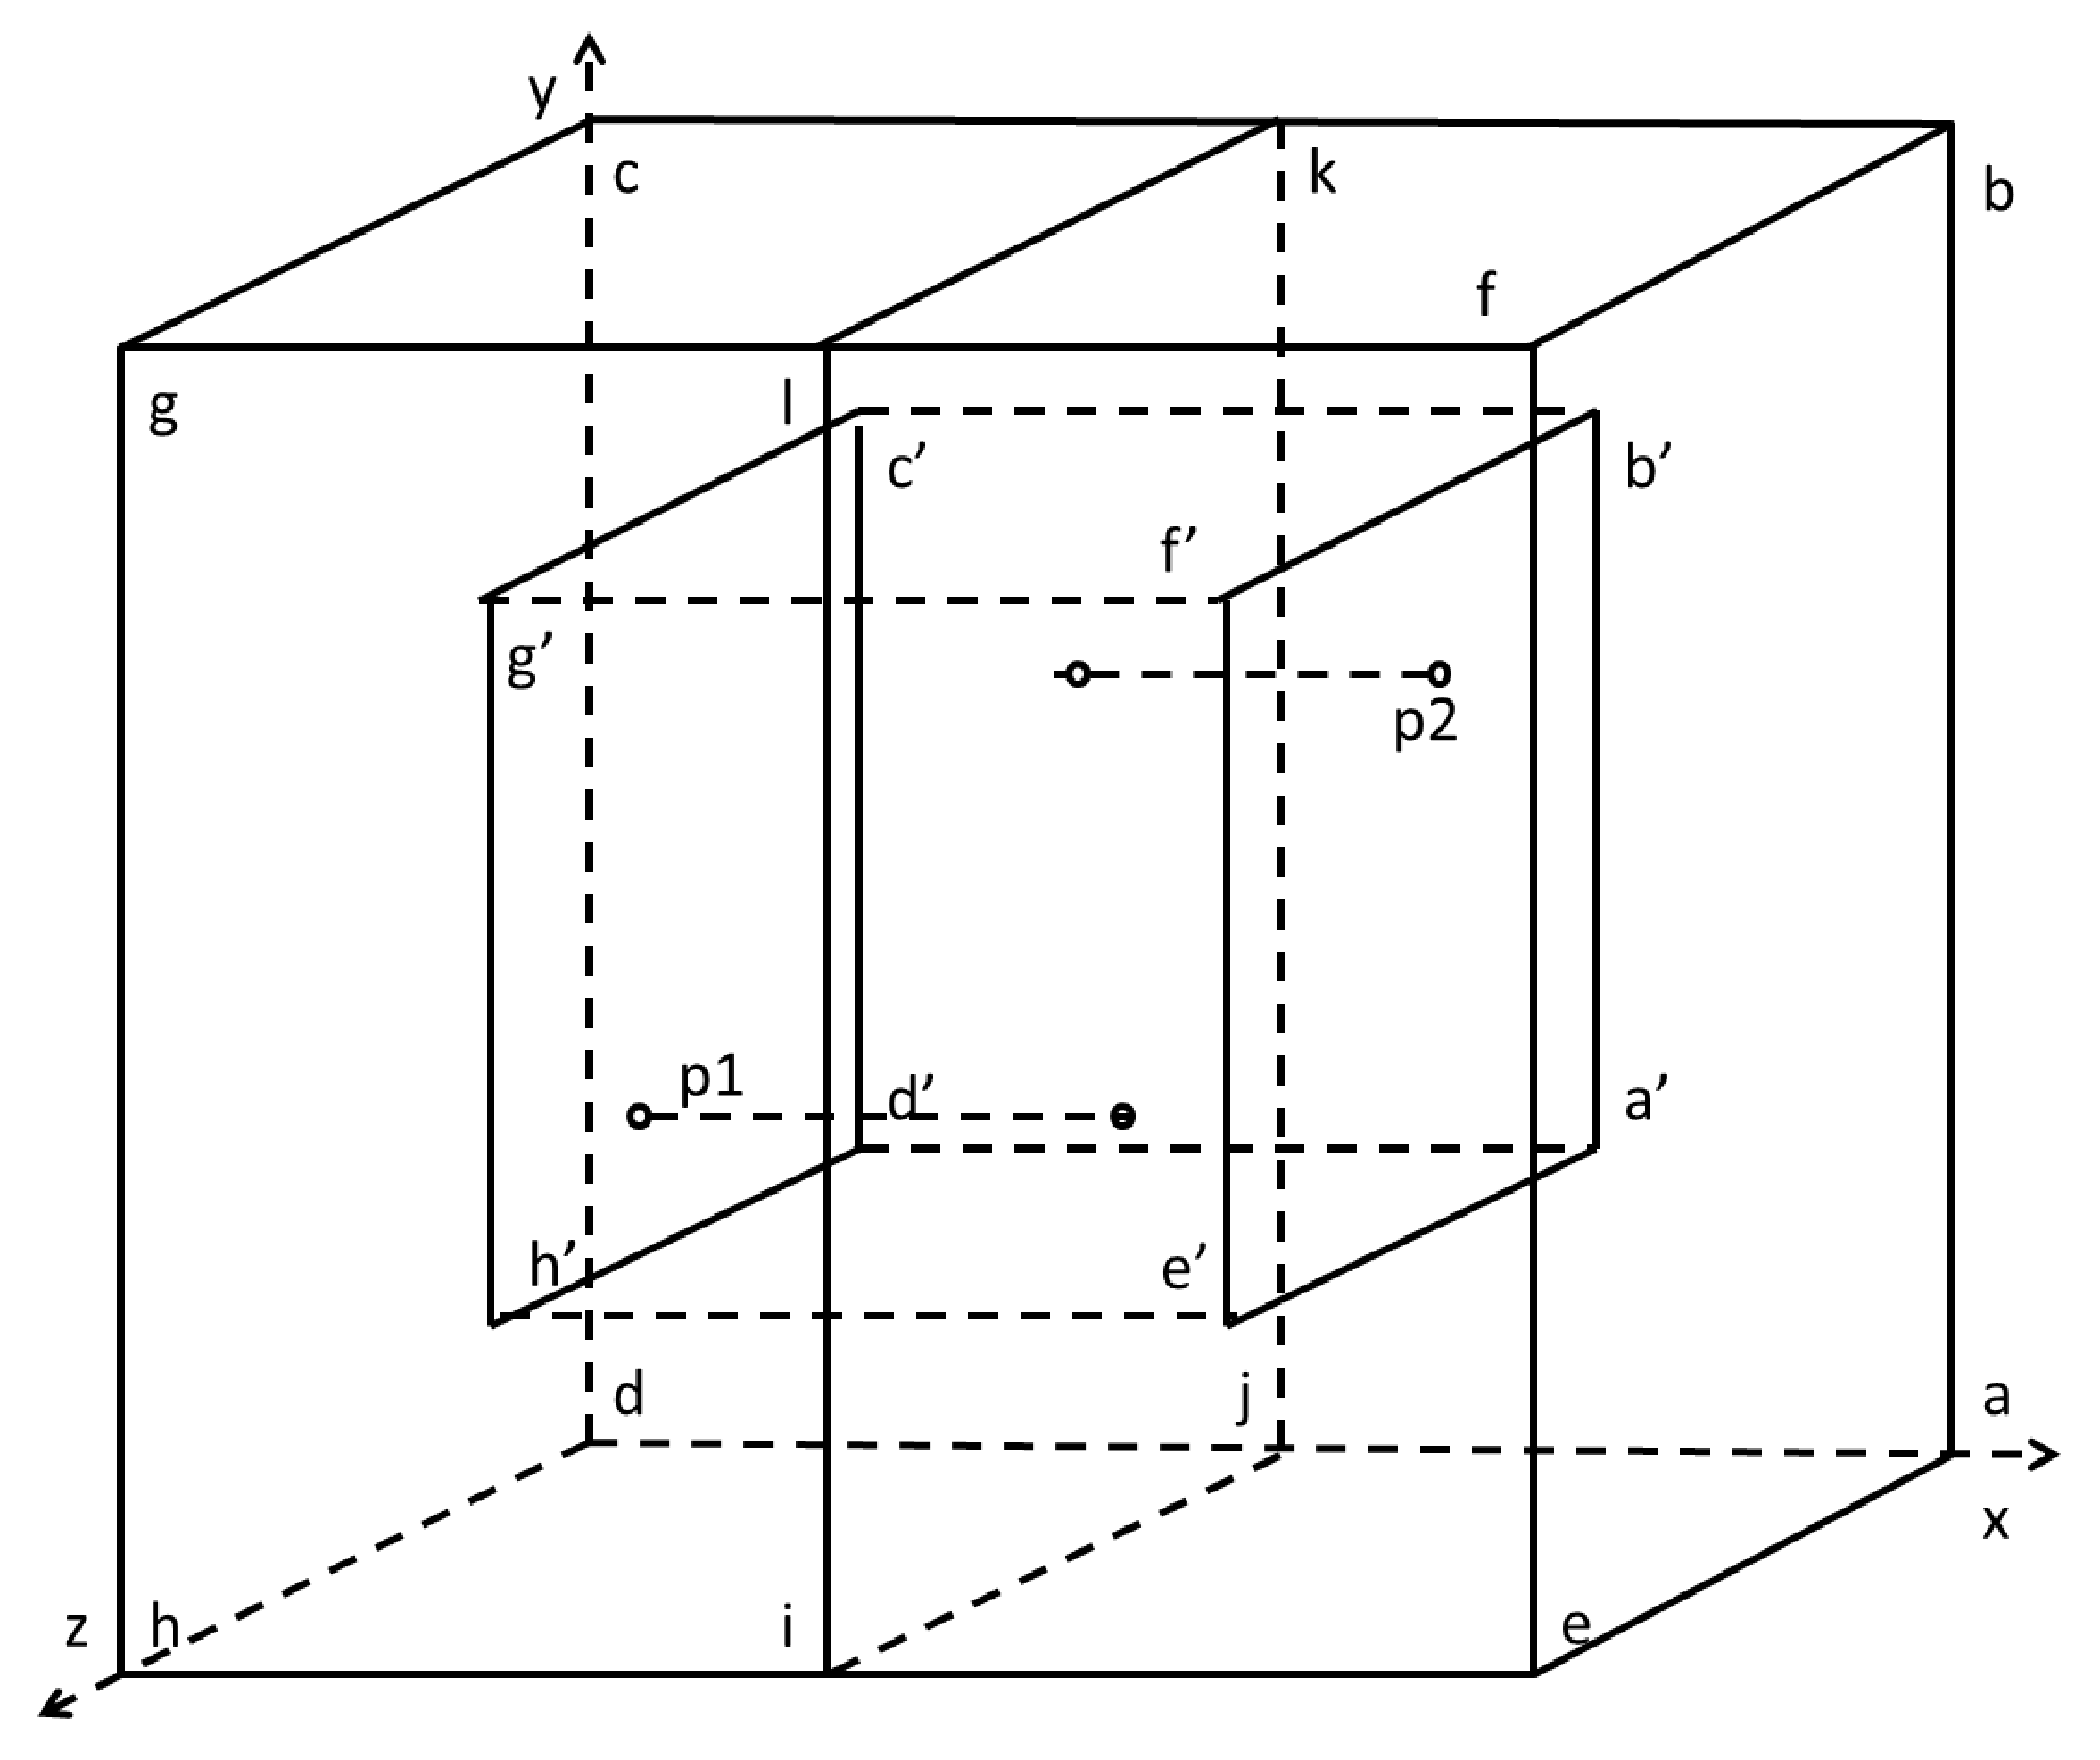
\includegraphics[width=2.5in]{figures/init_3D.eps}
\label{fig:threed}
\end{figure}

The $3$-D initial algorithm for orthogonal range query is pretty
straightforward and diagramed in \figref{threed}. Instead of center line,
we now have a center plane. In \figref{threed}, assuming $\id{x}$ is the
longest dimension and the first to reduce, we have a center face $\Box
\id{ijkl}$ to partition the entire grid into two parts. All the points
on the left-hand/right-hand side will reduce from center plane to itself
and store it as $\id{prefix/suffix\_grid}$. All the query range spanning
across the center plane can now be answered by two $2$-D queries. Then
recurse on both left and right parts of the center plane will cover all
$3$-D query ranges.

The meta-algorithm for $3$-D is also similar to the case of $2$-D, we
just need to reduce on all three dimensions to bring the preprocessing
complexity from $O(n_1 n_2 n_3 f(n_1) f(n_2) f(n_3))$ down to $O(n_1
n_2 n_3 f^*(n_1) f^*(n_2) f^*(n_3))$. The exact procedure is omitted
here.

\subsecput{init-2D}{Pseudo-code for the $2$-D initial algorithm}

\begin{figure}[!ht]
\small
\begin{codebox}
\Procname{$\proc{Init-2D}(\id{grid}, \id{x_0}, \id{x_1}, \id{y_0}, \id{y_1}; \proc{input\_1D\_algo}, \proc{op})$}
\li     $prefix\_grid \gets$ \New $((\id{x_1} - \id{x_0}) * (\id{y_1} - \id{y_0})$
\li     $suffix\_grid \gets$ \New $((\id{x_1} - \id{x_0}) * (\id{y_1} - \id{y_0})$
\li     \Comment Assuming we apply divide-and-conquer on dimension \id{x}
\li     \If $\id{x_1} - \id{x_0} <= 1$
\li         \Then \Return \Comment if the size of longer dimension $ <= 1$ then return
\li         \Else 
\li              $mid\_point \gets (\id{x_0} + \id{x_1})/2$
\li              \Comment Copy the starting point of prefix (on the right side of $mid\_point$)
\li              \Comment and suffix (on the left side of $mid\_point$)
\li              \For $y \gets \id{y_0}$ \To $\id{y_1}$
\li                  \Do $\id{suffix\_grid}[mid\_point-1][y] \gets \id{grid}[mid\_pont-1][y]$
\li                      $\id{prefix\_grid}[mid\_point][y] \gets \id{grid}[mid\_point][y]$ \End
\li              \Comment Reduce on all suffix
\li              \For $x \gets mid\_point-2$ \Downto $x_0$ 
\li                  \Do \For $y \gets \id{y_0}$ \To $\id{y_1}$
\li                      \Do $\id{suffix\_grid}[x][y] \gets \proc{op}(\id{grid}[x][y], \id{suffix\_grid}[x+1][y])$ \End \End
\li              \Comment Reduce on all prefix
\li              \For $x \gets mid\_point+1$ \To $x_1$
\li                  \Do \For $y \gets \id{y_0}$ \To $\id{y_1}$
\li                      \Do $\id{prefix\_grid}[x][y] \gets \proc{op}(\id{prefix\_grid}[x-1][y], \id{grid}[x][y])$ \End \End
\li              \Comment Apply the input $1$D algorithm on reduced prefix/suffix grid
\li              \Parfor $x \gets \id{x_0}$ \To $\id{x_1}$
\li                  \Do $\proc{input\_1D\_algo}(\id{suffix\_grid}[x][], \id{y_0}, \id{y_1}, \id{op})$
\li                      $\proc{input\_1D\_algo}(\id{prefix\_grid}[x][], \id{y_0}, \id{y_1}, \id{op})$ \End
\li              \Comment Recursively call \id{Init-2D} algorithm on the left side
\li              \Spawn $\proc{Init-2D}(\id{grid}, \id{x_0}, \id{mid\_point-1}, \id{y_0}, \id{y_1}; \id{input\_1D\_algo}, \id{op})$ 
\li              \Comment Recursively call \proc{Init-2D} algorithm on the right side
\li                     $\proc{Init-2D}(\id{grid}, \id{mid\_point}, \id{x_1}, \id{y_0}, \id{y_1}; \id{input\_1D\_algo}, \id{op})$ 
\li              \Sync \End
\end{codebox}
\caption{Initial $2$-D algorithm}
\label{fig:init-2D-algo}
\end{figure}

\subsecput{apdx-meta-2D}{Pseudo-code for the $2$-D meta algorithm}

% May put pseudo-code into appendix??
\begin{figure}[!ht]
\small
\begin{codebox}
\Procname{$\proc{Meta-2D}(\id{grid}, \id{x_0}, \id{x_1}, \id{y_0}, \id{y_1}; \id{REC}, \proc{input\_2D\_algo}, \proc{input\_1D\_algo}, \proc{op})$}
\li     \Comment Asssuming we do the data reduction on dimension $\id{x}$
\li     $seg\_size \gets \log(\id{x_1} - \id{x_0})$
\li     \Comment Depending on $\id{REC}$ level, we partition the seg\_size into $\log (\id{x_1} - \id{x_0})$, or $\log^* (\id{x_1} - \id{x_0})$, $\log^{**} (\id{x_1} - \id{x_0})$, $\ldots$
\li     \For $i \gets 0$ \To $REC$ 
\li         \Do $seg\_size \gets * seg\_size$ \End
\li     $n\_segs \gets (\id{x_1} - \id{x_0})/seg\_size$
\li     $promoted\_grid \gets $ \New $(n\_segs * (\id{y_1} - \id{y_0}))$
\li     $prefix\_grid \gets $ \New $((\id{x_1} - \id{x_0}) * (\id{y_1} - \id{y_0}))$
\li     $suffix\_grid \gets $ \New $((\id{x_1} - \id{x_0}) * (\id{y_1} - \id{y_0}))$
\li     \For $i \gets 0$ \To $n\_segs$
\li         \Do \For $j \gets 0$ \To $\id{y_1} - \id{y_0}$
\li             \Do \Comment $\proc{Reduce}$ apply input partial sum operator $\proc{op}$ over range $[i*seg_size, (i+1)*seg_size][j]$ 
\zi                 \Comment and return the reduced result into $promoted\_grid[i][j]$
\li                 $promoted\_grid[i][j] \gets \proc{Reduce}(i, j, \proc{op})$ 
\li                 \Comment $\proc{Reduce\_prefix}$ apply input partial sum operator $\proc{op}$ over range $[i*seg\_size, (i+1)*seg\_size][j]$ 
\zi                 \Comment and reduce the data relative to the beginning point of the segment ($i*seg_size$)
\li                 $prefix\_grid[i][j] \gets \proc{Reduce\_prefix}(i, j, \proc{op})$
\li                 \Comment $\proc{Reduce\_suffix}$ apply input partial sum operator $\proc{op}$ over range $[i*seg\_size, (i+1)*seg\_size][j]$ 
\zi                 \Comment and reduce the data relative to the end point of the segment ($(i+1)*seg_size$)
\li                 $suffix\_grid[i][j] \gets \proc{Reduce\_suffix}(i, j, \proc{op})$ \End \End
\li     \Comment Apply \proc{input\_2D\_algo} on the $promoted\_grid$
\li     $\proc{input\_2D\_algo}(promoted_grid, 0, n_segs, \id{y_0}, \id{y_1}; \id{REC-1}, \proc{input\_1D\_algo}, \proc{op})$
\li     \Parfor $i \gets 0$ \To $n\_segs$
\li         \Do \Comment Apply \proc{Meta-2D} itself onto the segments of $[i * seg\_size, (i+1) * seg\_size, \id{y_0}, \id{y_1}]$
\li             $\proc{Meta-2D}(\id{grid}, i * seg\_size, (i+1) * seg\_size, \id{y_0}, \id{y_1}; \id{REC}, \proc{input\_2D\_algo}, \proc{input\_1D\_algo}, \proc{op})$ \End
\li     \Parfor $i \gets \id{x_0}$ \To $\id{x_1}$
\li         \Do \Comment Apply the input $1$D algorithm on reduced prefix/suffix grid
\li             $\proc{input\_1D\_algo}(prefix\_grid[i], \id{y_0}, \id{y_1}, \proc{op})$
\li             $\proc{input\_1D\_algo}(suffix\_grid[i], \id{y_0}, \id{y_1}, \proc{op})$ \End
\end{codebox}
\caption{Meta $2$-D algorithm}
\label{fig:meta-2D-algo}
\end{figure}

\subsecput{apdx-meta-non-orthogonal}{Supplemental material for meta-algorithm for non-orthogonal range queries}

\begin{figure*}[t!]
\centering
\includegraphics[width=3in]{figures/meta_right_triangle.eps}
\vspace{-2cm}
\label{fig:meta-right-triangle}
\caption{Meta-algorithm for right triangular query in $2$-D grid.}
\end{figure*}

\subsecput{apdx-expr}{Experimental results of static partial sum problem}
\begin{figure*}[!ht]
\centering
\subfigure[Preprocessing time of meta-algorithm for $1$-D grid.]{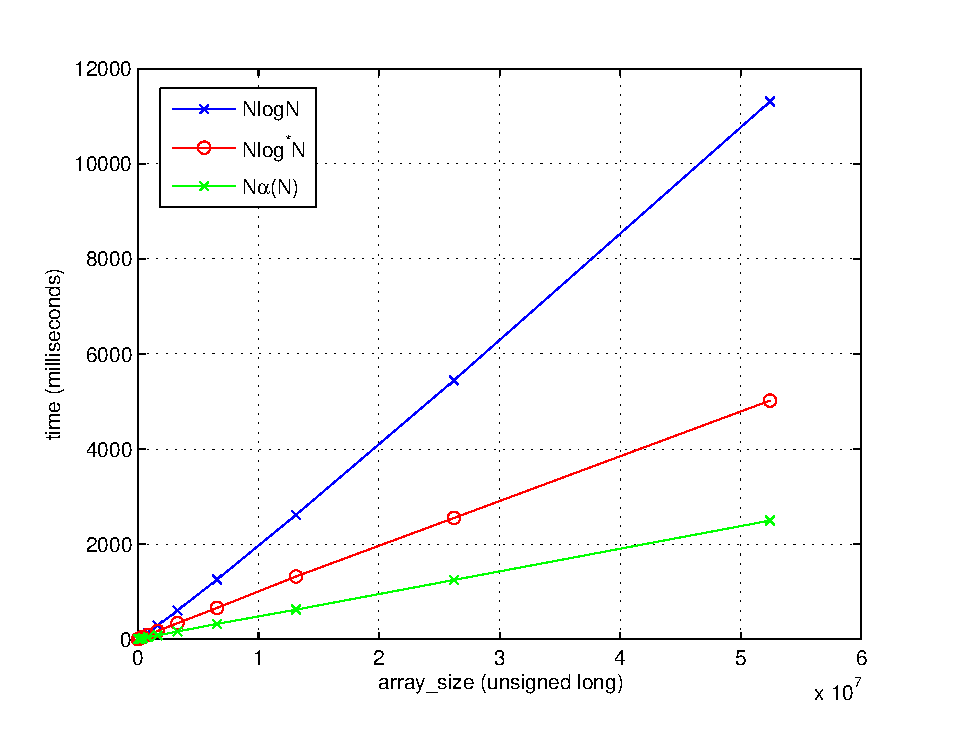
\includegraphics[clip,width=3in]{figures/meta_1D_PP.eps}
\label{fig:meta-1D-PP}}
\hfill
%\hspace{0.01cm}
\subfigure[Preprocessing time of meta-algorithm for $2$-D grid]{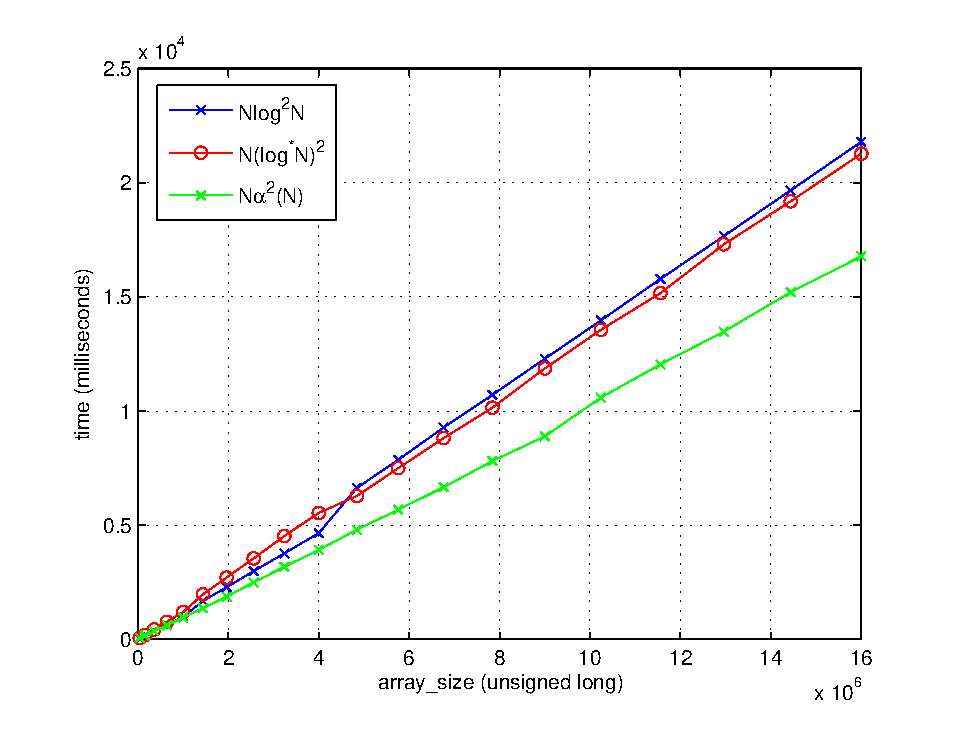
\includegraphics[clip,width=3in]{figures/meta_2D_PP.eps}
\label{fig:meta-2D-PP}
}
\caption{Performance data of meta-algorithm's Preprocessing time for $1$-D and $2$-D grid}
\label{fig:meta-PP}
\end{figure*}

\begin{figure*}[!ht]
\centering
\subfigure[Query time of meta-algorithm for $1$-D grid]{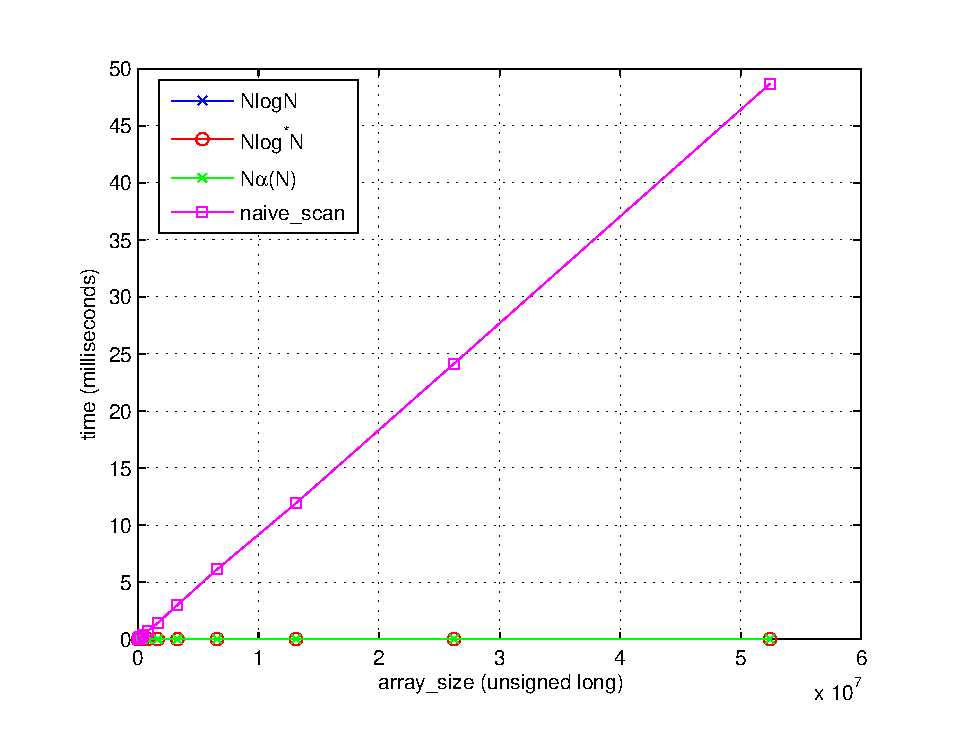
\includegraphics[clip,width=3in]{figures/meta_1D_query.eps}
\label{fig:meta-1D-query}}
\hfill
%\hspace{0.01cm}
\subfigure[Query time of meta-algorithm for $2$-D grid]{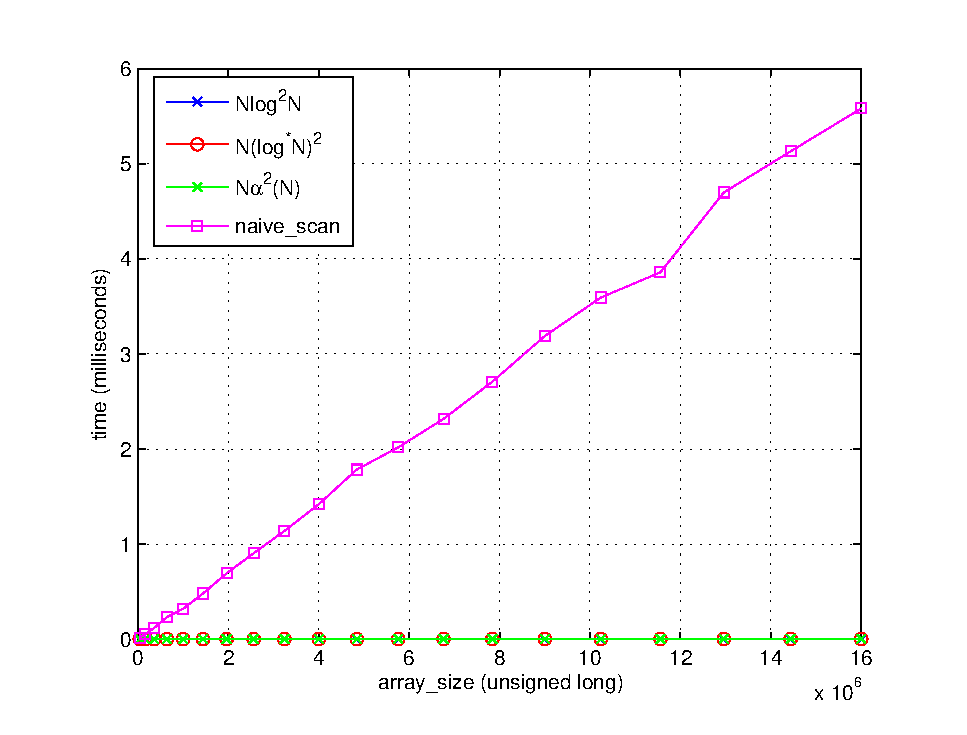
\includegraphics[clip,width=3in]{figures/meta_2D_query.eps}
\label{fig:meta-2D-query}
}
\caption{Performance data of meta-algorithm's Query time for $1$-D and $2$-D grid}
\label{fig:meta-query}
\end{figure*}




\end{document}

